% Options for packages loaded elsewhere
\PassOptionsToPackage{unicode}{hyperref}
\PassOptionsToPackage{hyphens}{url}
%
\documentclass[
  10pt,
  ignorenonframetext,
]{beamer}
\usepackage{pgfpages}
\setbeamertemplate{caption}[numbered]
\setbeamertemplate{caption label separator}{: }
\setbeamercolor{caption name}{fg=normal text.fg}
\beamertemplatenavigationsymbolsempty
% Prevent slide breaks in the middle of a paragraph
\widowpenalties 1 10000
\raggedbottom
\setbeamertemplate{part page}{
  \centering
  \begin{beamercolorbox}[sep=16pt,center]{part title}
    \usebeamerfont{part title}\insertpart\par
  \end{beamercolorbox}
}
\setbeamertemplate{section page}{
  \centering
  \begin{beamercolorbox}[sep=12pt,center]{section title}
    \usebeamerfont{section title}\insertsection\par
  \end{beamercolorbox}
}
\setbeamertemplate{subsection page}{
  \centering
  \begin{beamercolorbox}[sep=8pt,center]{subsection title}
    \usebeamerfont{subsection title}\insertsubsection\par
  \end{beamercolorbox}
}
\AtBeginPart{
  \frame{\partpage}
}
\AtBeginSection{
  \ifbibliography
  \else
    \frame{\sectionpage}
  \fi
}
\AtBeginSubsection{
  \frame{\subsectionpage}
}
\usepackage{amsmath,amssymb}
\usepackage{iftex}
\ifPDFTeX
  \usepackage[T1]{fontenc}
  \usepackage[utf8]{inputenc}
  \usepackage{textcomp} % provide euro and other symbols
\else % if luatex or xetex
  \usepackage{unicode-math} % this also loads fontspec
  \defaultfontfeatures{Scale=MatchLowercase}
  \defaultfontfeatures[\rmfamily]{Ligatures=TeX,Scale=1}
\fi
\usepackage{lmodern}
\ifPDFTeX\else
  % xetex/luatex font selection
\fi
% Use upquote if available, for straight quotes in verbatim environments
\IfFileExists{upquote.sty}{\usepackage{upquote}}{}
\IfFileExists{microtype.sty}{% use microtype if available
  \usepackage[]{microtype}
  \UseMicrotypeSet[protrusion]{basicmath} % disable protrusion for tt fonts
}{}
\makeatletter
\@ifundefined{KOMAClassName}{% if non-KOMA class
  \IfFileExists{parskip.sty}{%
    \usepackage{parskip}
  }{% else
    \setlength{\parindent}{0pt}
    \setlength{\parskip}{6pt plus 2pt minus 1pt}}
}{% if KOMA class
  \KOMAoptions{parskip=half}}
\makeatother
\usepackage{xcolor}
\newif\ifbibliography
\setlength{\emergencystretch}{3em} % prevent overfull lines
\providecommand{\tightlist}{%
  \setlength{\itemsep}{0pt}\setlength{\parskip}{0pt}}
\setcounter{secnumdepth}{-\maxdimen} % remove section numbering
\usepackage{booktabs}

\usepackage{color, colortbl}
\definecolor{Gray}{gray}{0.9}

\def\begincols{\begin{columns}}
\def\begincol{\begin{column}}
\def\endcol{\end{column}}
\def\endcols{\end{columns}}

\setbeamertemplate{caption}[numbered]
\setbeamertemplate{itemize items}[default]
\setbeamertemplate{itemize subitem}[circle]

\usepackage{ctex} % CJK 包
%\usepackage{xeCJK}
%\setCJKmainfont[AutoFakeBold = {2.25}]{SimSum}

\logo{
\includegraphics[scale=0.2]{bbk200}}
%\usetheme{Madrid}
%\usefonttheme{serif}

%\pgfdeclareimage[scale=0.2]{logo}{bbk2}
%\logo{\pgfuseimage{logo}}

% \begincols
% \begincol{.48\textwidth}
% \endcol
% \begincol{.48\textwidth}
% \endcol
% \endcols

% How many criminal candidates were there? Where and when?
% 6,499 out of 35,075 contesting candidates -- close to 20\%

% Did criminal candidates win elections? Where and when?
% Given that a candidate is a criminal, the probability of winning the election is about 0.22; in contrast, Given that a candidate is NOT a criminal, the probability of winning the election is about 0.12. (X)

% How many criminal politicians were there? Where and when? 

% Party affiliations: BJP (23\%), Congress (18\%), 
\usepackage{bookmark}
\IfFileExists{xurl.sty}{\usepackage{xurl}}{} % add URL line breaks if available
\urlstyle{same}
\hypersetup{
  hidelinks,
  pdfcreator={LaTeX via pandoc}}

\title{\hfill\break
\hfill\break
Using Numbers to Study Contemporary China\\
\strut \\}
\author{Dr Chao-Yo Cheng\\
\strut \\
(Birkbeck, University of London)}
\date{}

\begin{document}
\frame{\titlepage}

\begin{frame}{Using numbers to study China}
\phantomsection\label{using-numbers-to-study-china}
\begincols
  \begincol{.4\textwidth}
    \vspace{0.4cm}
    \begin{figure}
    \centering
    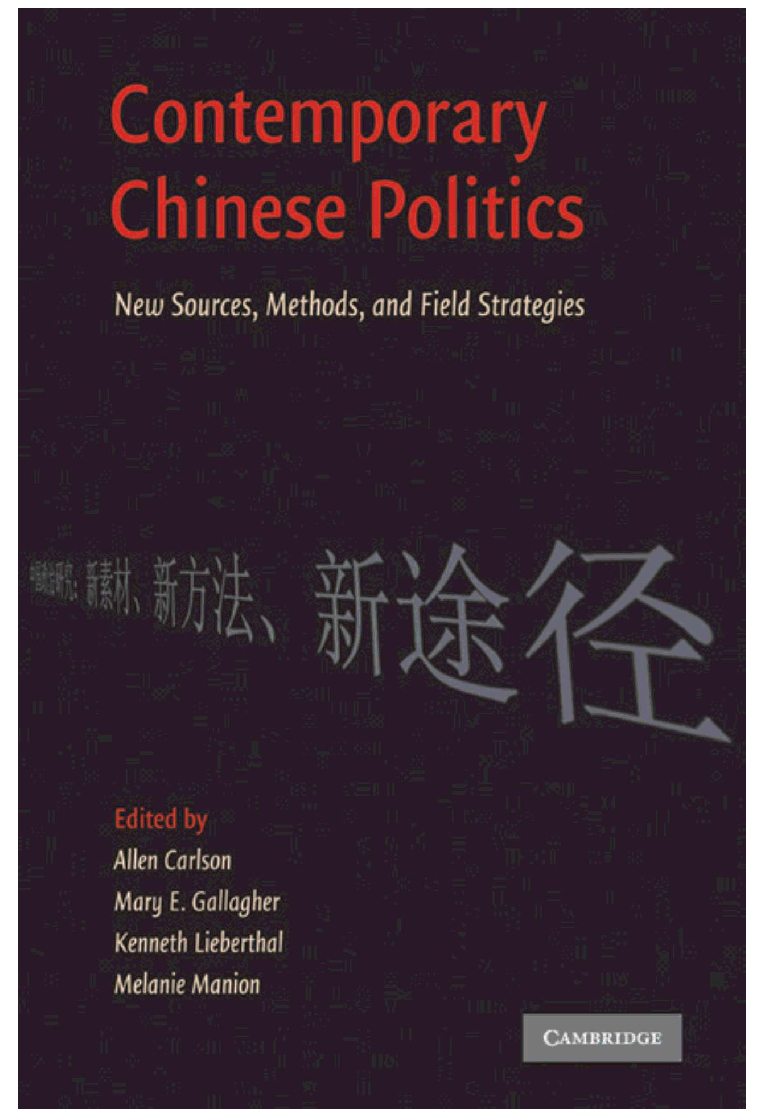
\includegraphics[scale=0.35]{Figs/book_crop}
    \end{figure}
  \endcol
  \begincol{.5\textwidth}
  \hspace{0.3cm}
  \begin{itemize}
    \item Why "numbers" matter?
    \vspace{0.7cm}
    \item Where "data" comes from?
    \vspace{0.7cm}
    \item How should we work with data?
  \end{itemize}
  \endcol
\endcols
\end{frame}

\begin{frame}{Why numbers matter?}
\phantomsection\label{why-numbers-matter}
\begin{itemize}
\small
  \item The field of China studies has changed significantly as a result of \textbf{data availability} in digital forms and \textbf{methodological advances} 
  \vspace{0.1cm}
  \begin{itemize}
    \item Quant techniques are essential to \textbf{establish patterns} for theory building and policy impact evaluation
    \item Using numbers also encourage us to rethink the purpose of China studies -- area studies or comparative politics?
    \item The use of computational and quantitative data/methods by no means undermine the importance of traditional approaches -- \textbf{multi-method/data triangulation} is now the norm
  \end{itemize}
  \vspace{0.3cm}
  \item Changing \textbf{geopolitical environment} also prompts the computational or even quantitative turn in the study of contemporary China
\end{itemize}
\end{frame}

\begin{frame}
\vspace{0.4cm}

\begin{center}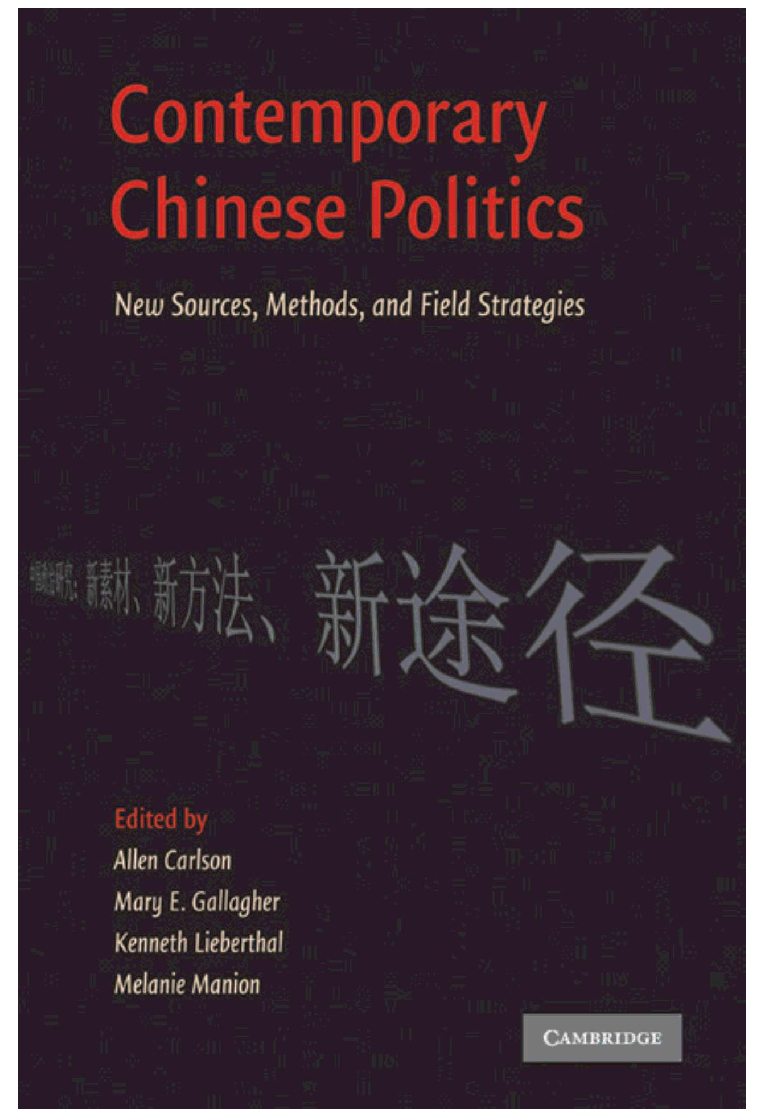
\includegraphics[width=0.35\linewidth]{Figs/book_crop} \end{center}
\vspace{0.2cm}
\begin{center}
\scriptsize
\textbf{Manion, Melanie (Duke), Kenneth Lieberthal (Michigan), Mary E. Gallagher (Michigan), and Allen Carlson (Cornell). 2010. \textit{Contemporary Chinese Politics: New Sources, Methods, and Field Strategies}. New York, NY: Cambridge University Press.}
\end{center}
\end{frame}

\begin{frame}{Where ``data'' comes from}
\phantomsection\label{where-data-comes-from}
\begin{itemize}
  \item Surveys, such as
  \vspace{0.1cm}
  \begin{itemize}
    \item Chinese General Social Survey (CGSS) -- Prof Xiaogang Wu (NYU Shanghai)
    \item China Family Panel Studies (CFPS) -- Prof Yu XIE (Princeton)
    \item Asianbarometer or World Values Survey (with caveats)
  \end{itemize}
  \vspace{0.2cm}
  \item Admin data, including socioeconomic surveys (e.g., statistical yearbooks 统计年鉴) and population census
  \vspace{0.2cm}
  \item Digital and "big" data, such as
  \vspace{0.1cm}
  \begin{itemize}
    \item Social media posts (e.g., Weibo)
    \item Search engine (e.g., Baidu Index) -- comparable to Google Trends
  \end{itemize}
\end{itemize}
\end{frame}

\begin{frame}
\vspace{0.4cm}

\begin{center}
\includegraphics[width=0.9\linewidth]{Figs/pkuverse_crop} \end{center}
\vspace{0.3cm}
\begin{center}
\textbf{\url{https://opendata.pku.edu.cn/}}
\end{center}
\end{frame}

\begin{frame}
\vspace{0.4cm}

\begin{center}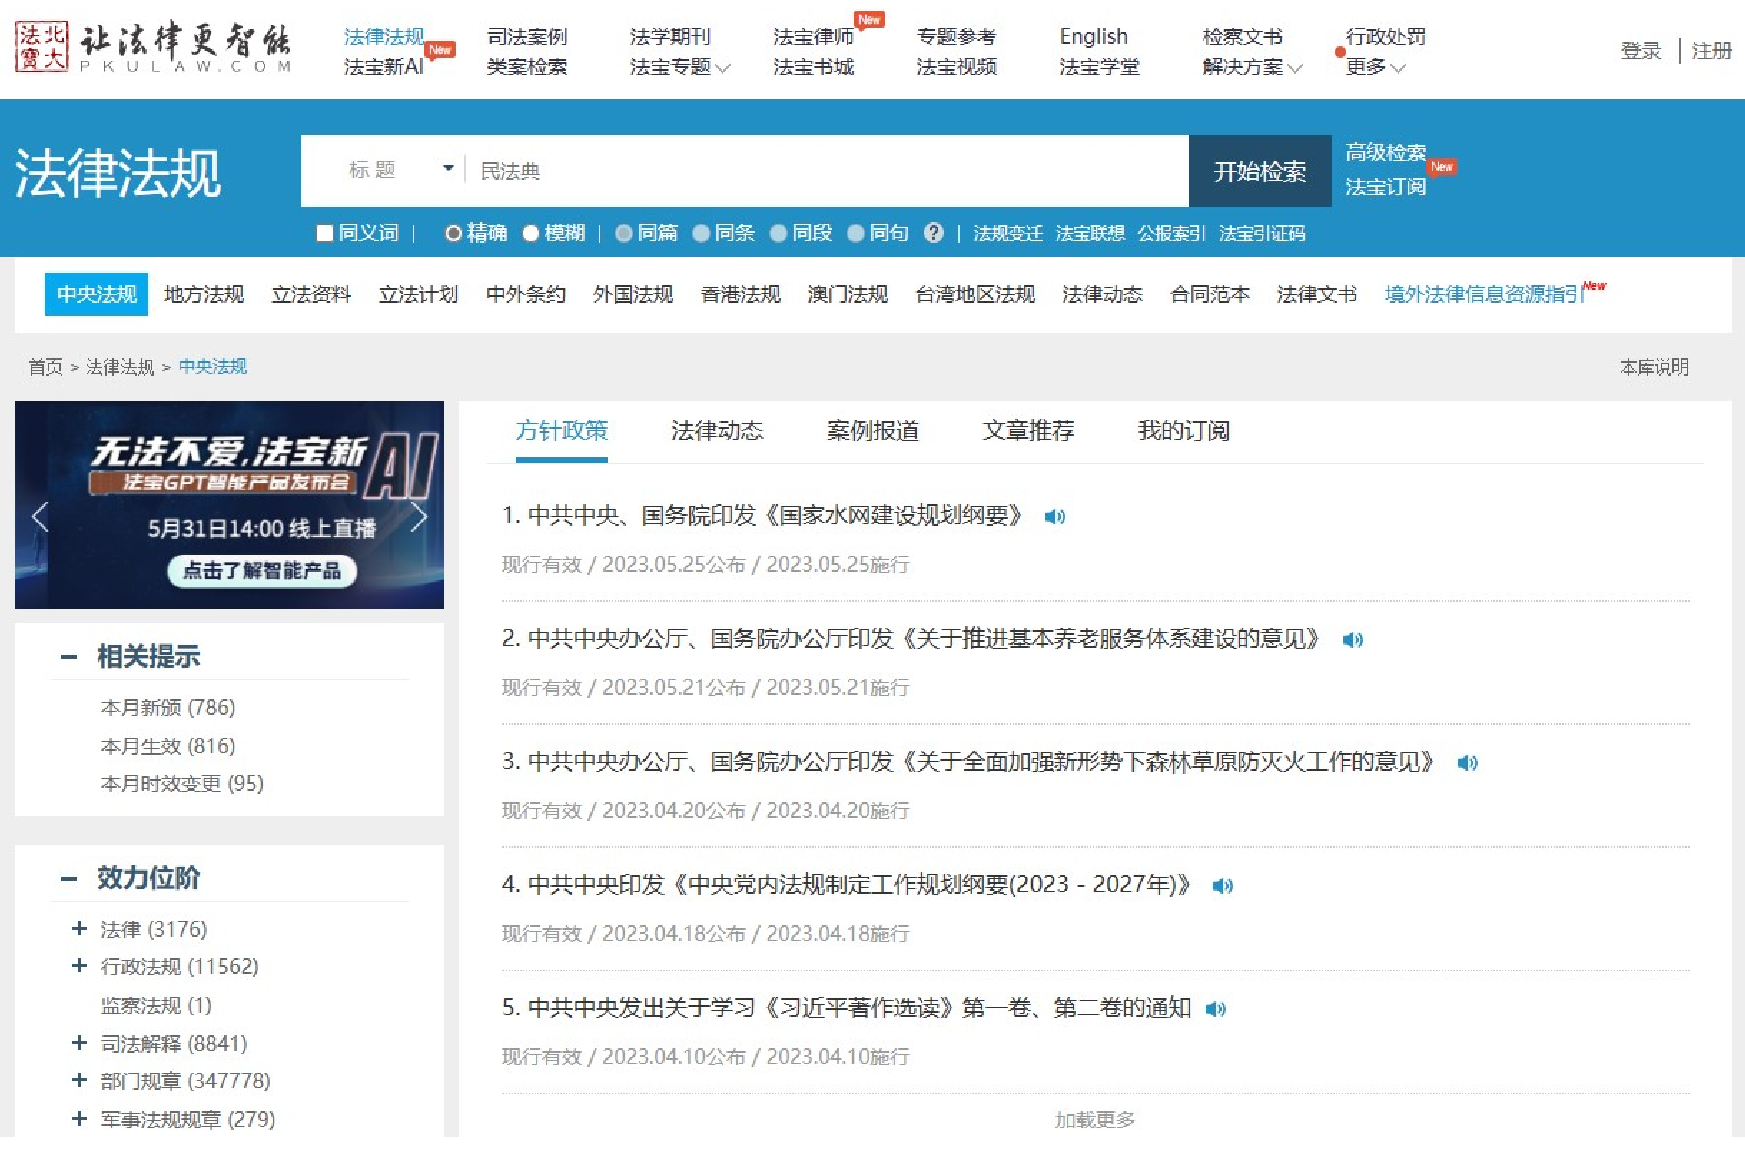
\includegraphics[width=0.9\linewidth]{Figs/pkulaw_crop} \end{center}
\vspace{0.3cm}
\begin{center}
\textbf{\url{https://www.pkulaw.net/}}
\end{center}
\end{frame}

\begin{frame}
\vspace{0.4cm}

\begin{center}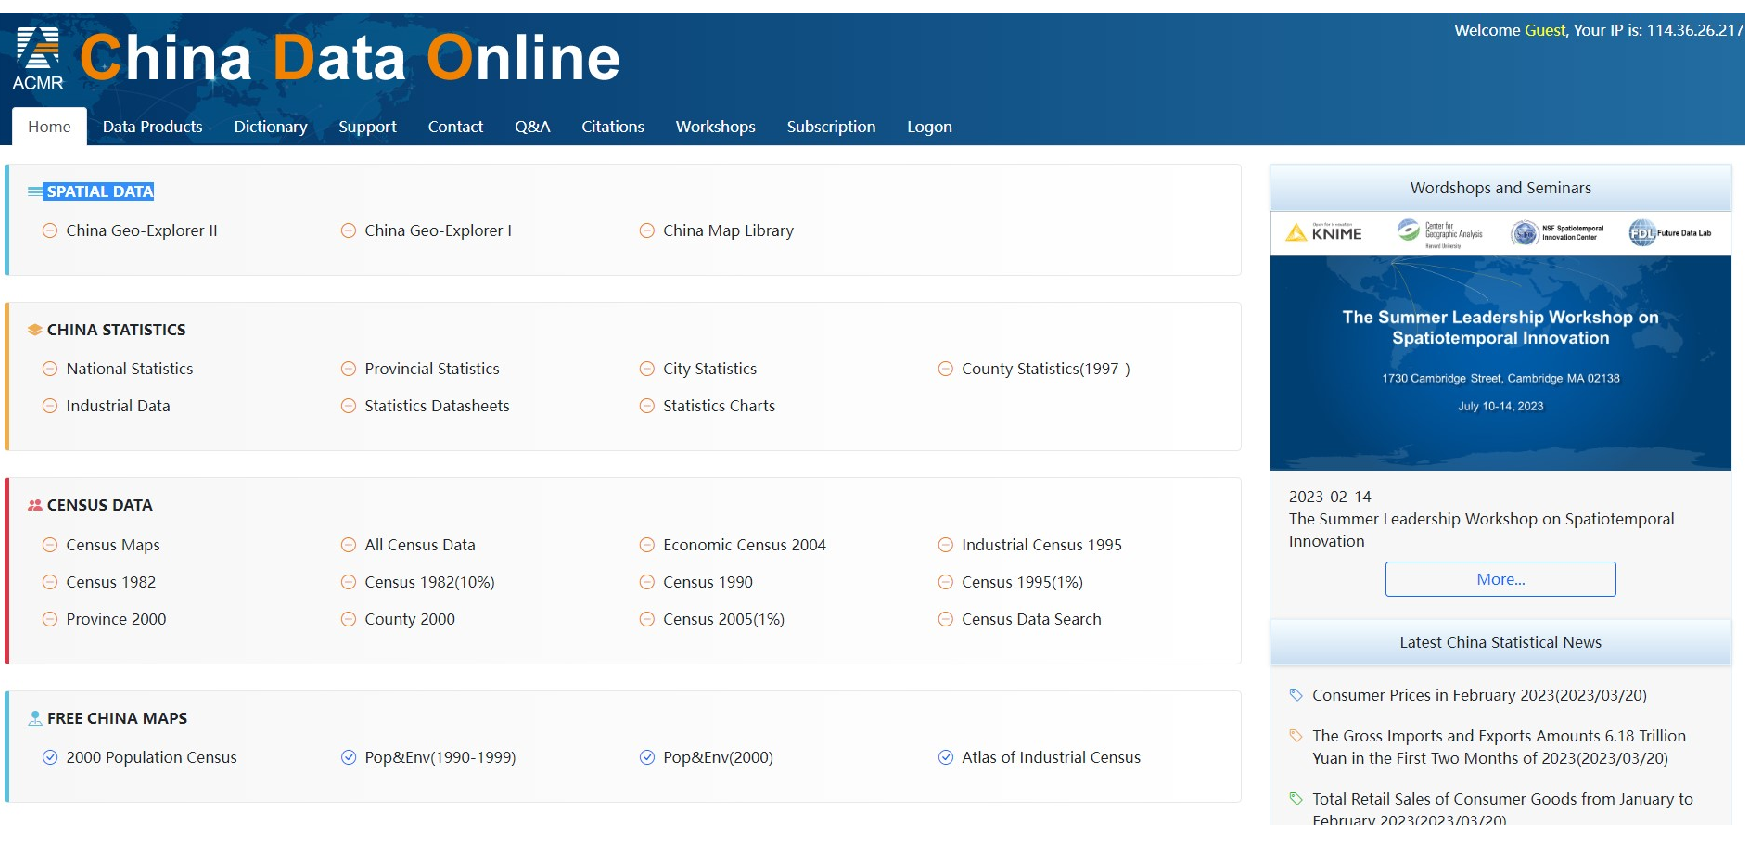
\includegraphics[width=0.9\linewidth]{Figs/cdo_crop} \end{center}
\vspace{0.3cm}
\begin{center}
\textbf{\url{https://www.china-data-online.com/}}
\end{center}
\end{frame}

\begin{frame}
\vspace{0.4cm}

\begin{center}
\includegraphics[width=0.9\linewidth]{Figs/baidu_crop} \end{center}
\vspace{0.3cm}
\begin{center}
\textbf{\url{https://index.baidu.com/}}
\end{center}
\end{frame}

\begin{frame}{Qualitative materials for empirical triangulation}
\phantomsection\label{qualitative-materials-for-empirical-triangulation}
\begin{itemize}
  \item Gazetteers (通志)
  \vspace{0.2cm}
  \item Yearbooks (年鉴), published yearly by various Party departments and government offices 
  \vspace{0.2cm}
  \item Culture and history materials (文史资料), published by the Chinese people's consultative conferences (政协)
  \vspace{0.2cm}
  \item Government work reports (政府工作报告), published by the people's governments
  \vspace{0.2cm}
  \item ... and so on so forth (e.g., archived historical materials compiled by the government or researchers)
\end{itemize}
\end{frame}

\begin{frame}
\begin{center}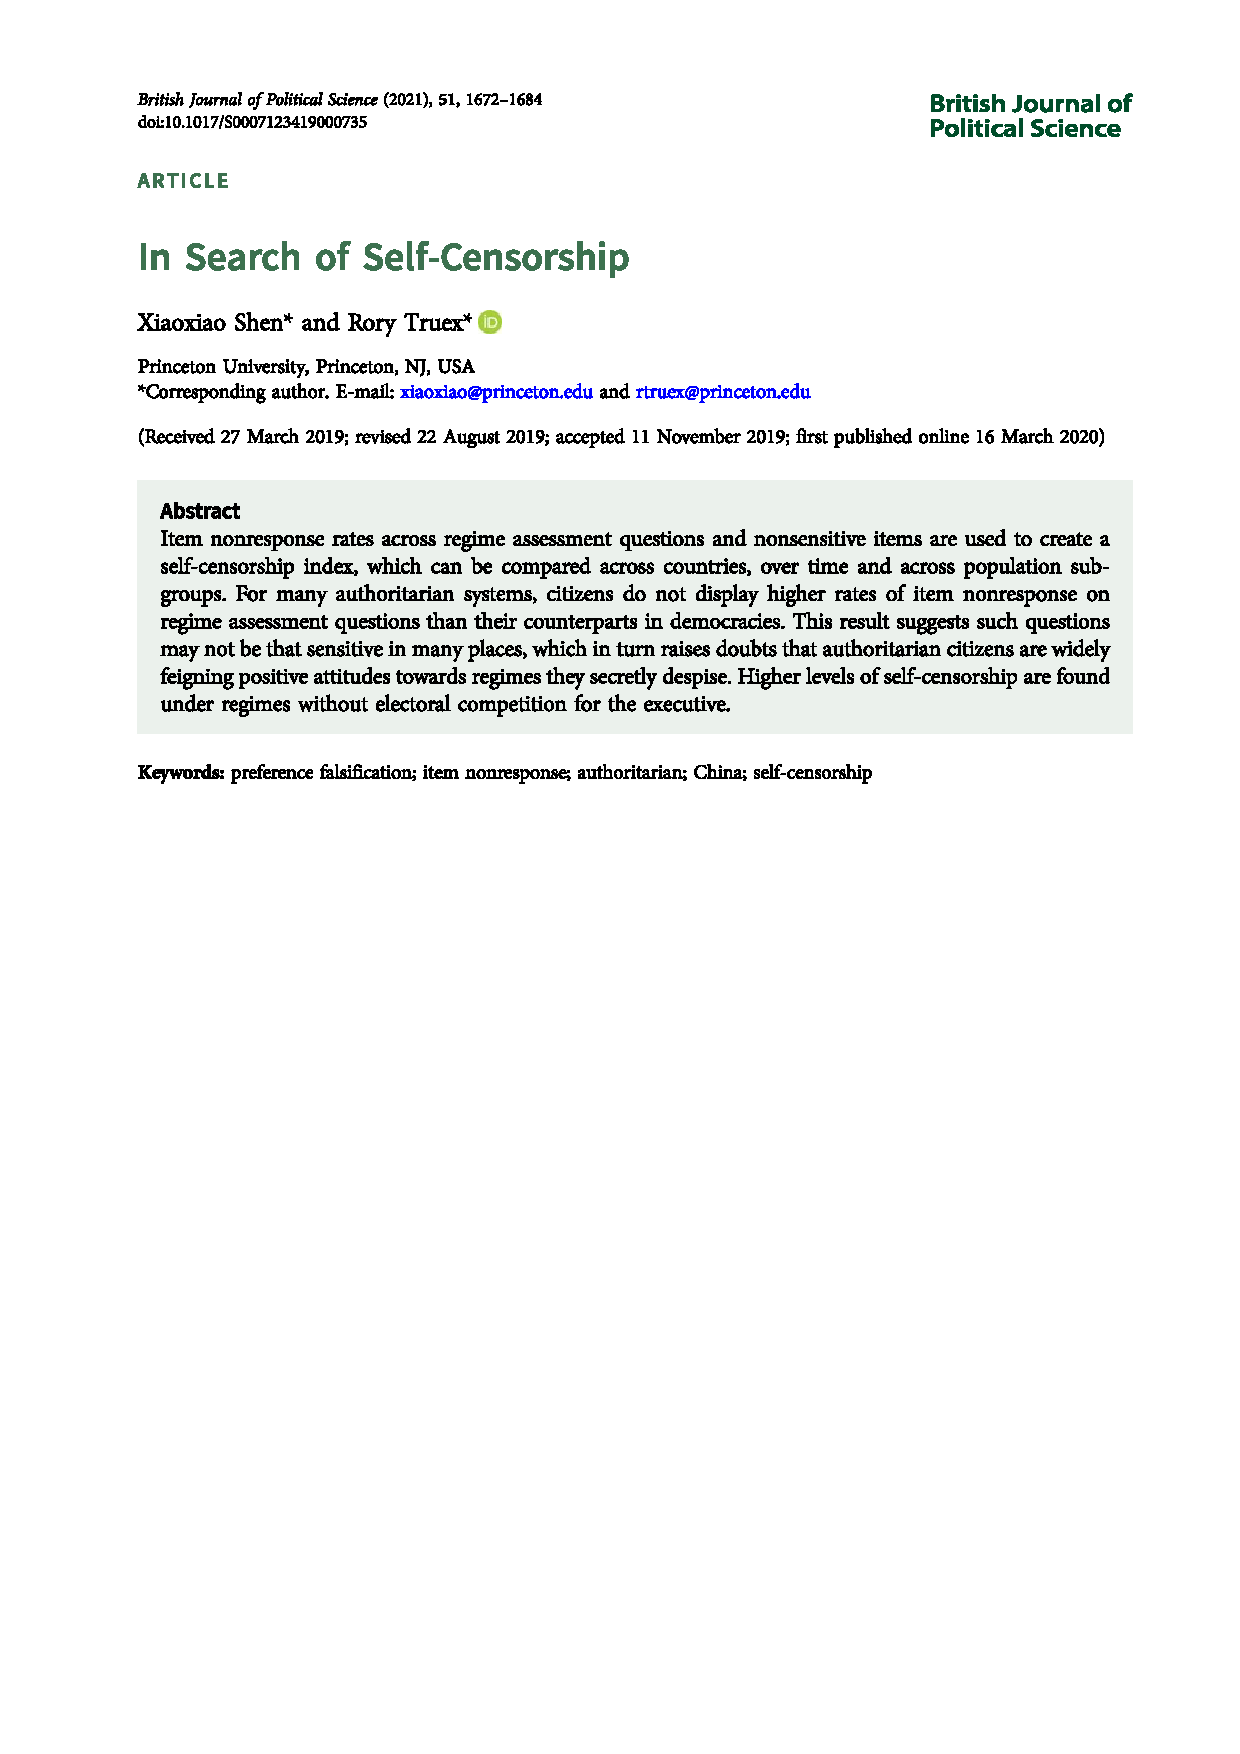
\includegraphics[width=0.9\linewidth]{Figs/Examples/truex_cover} \end{center}
\end{frame}

\begin{frame}
\begin{center}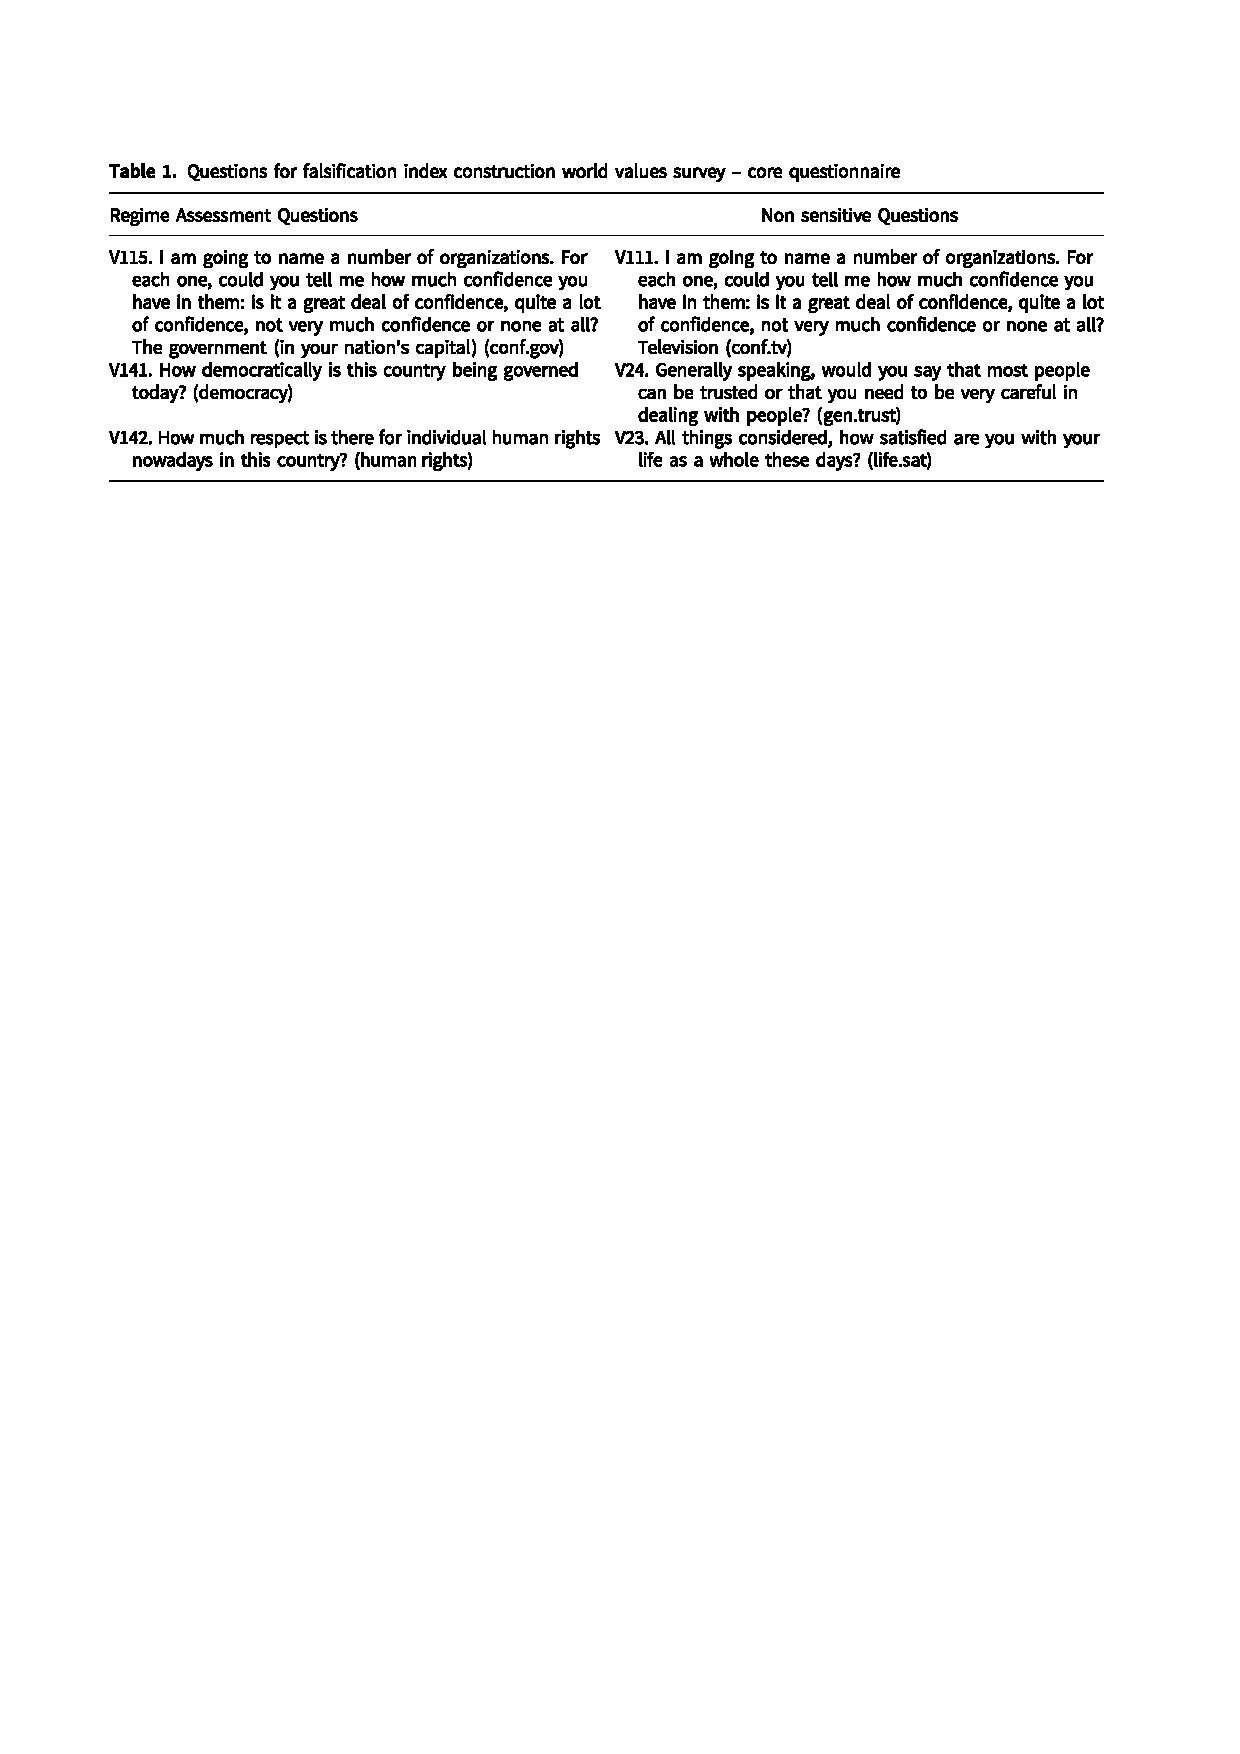
\includegraphics[width=0.9\linewidth]{Figs/Examples/truex_table} \end{center}
\end{frame}

\begin{frame}
\begin{center}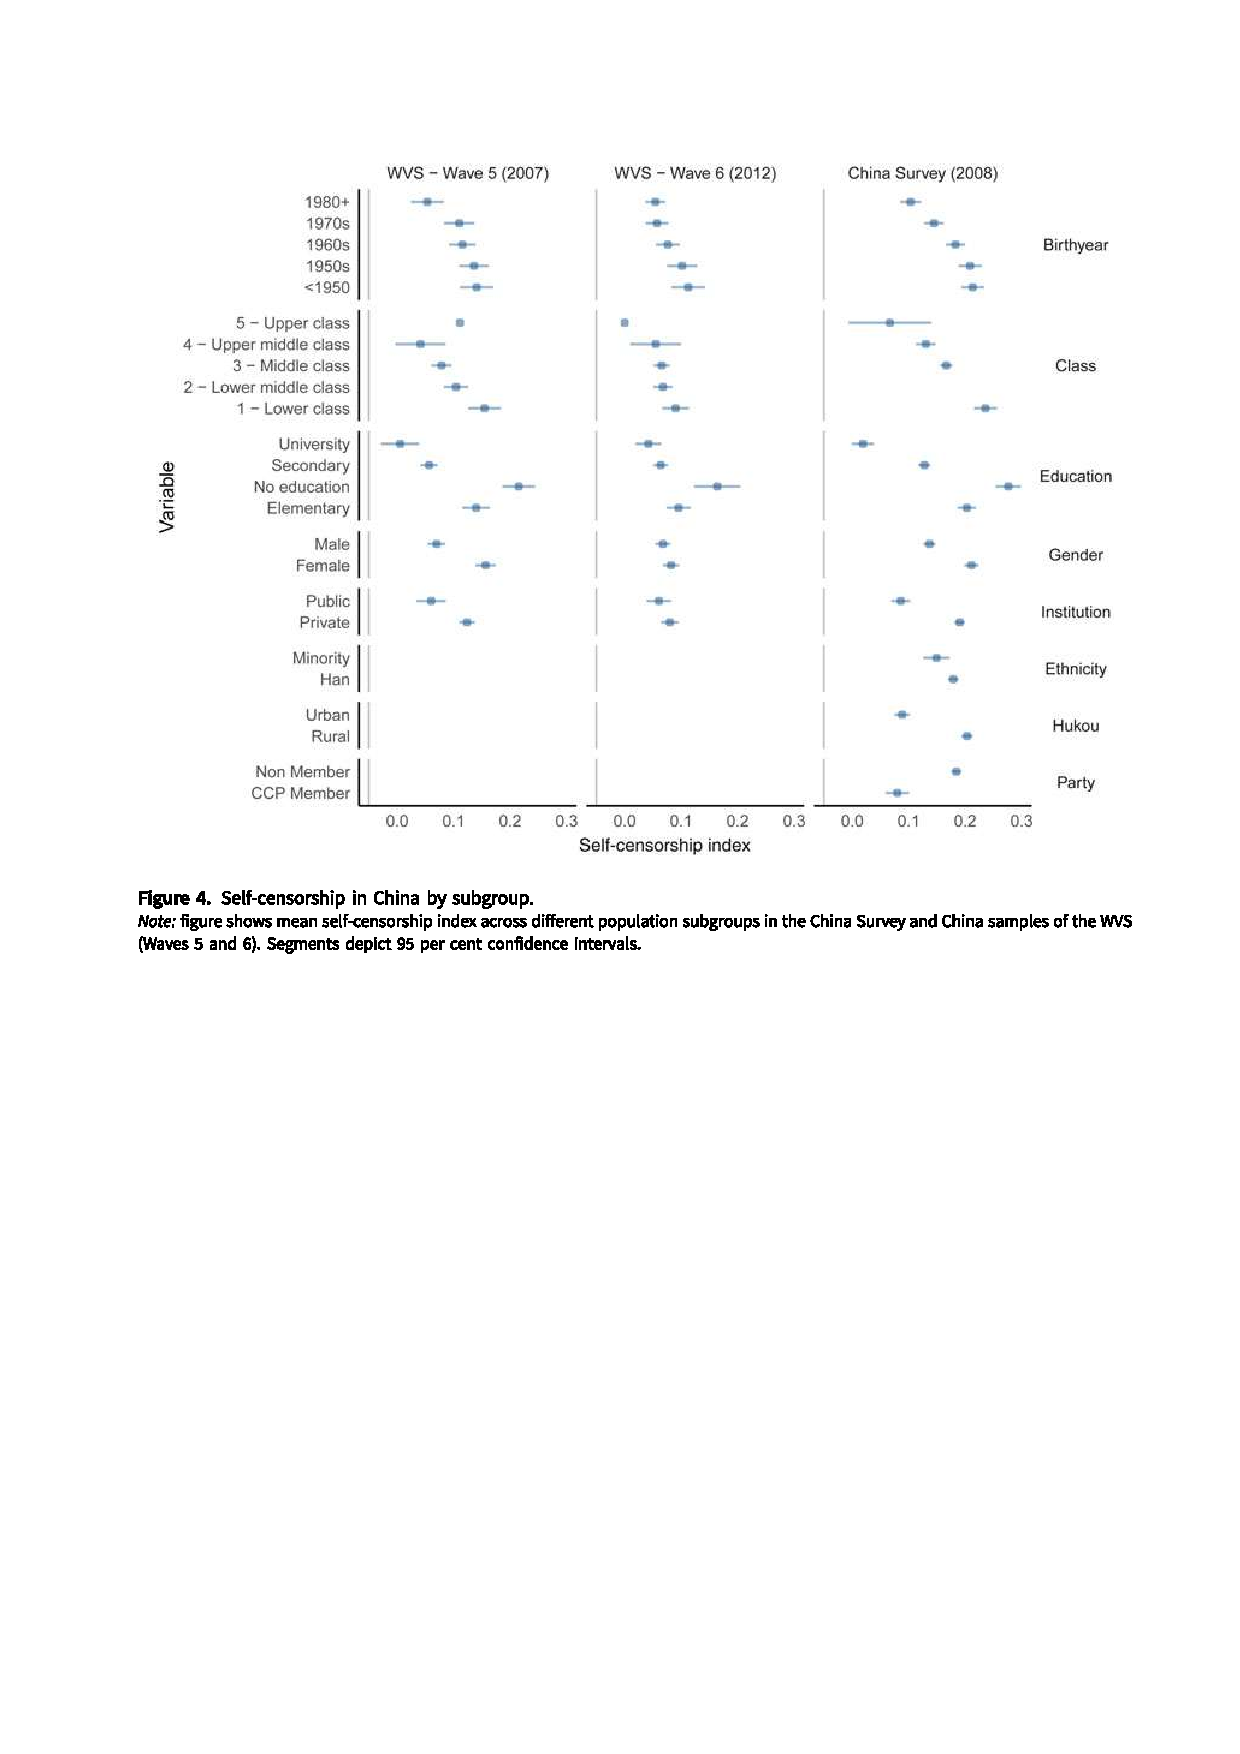
\includegraphics[width=0.9\linewidth]{Figs/Examples/truex_res} \end{center}
\end{frame}

\begin{frame}
\begin{center}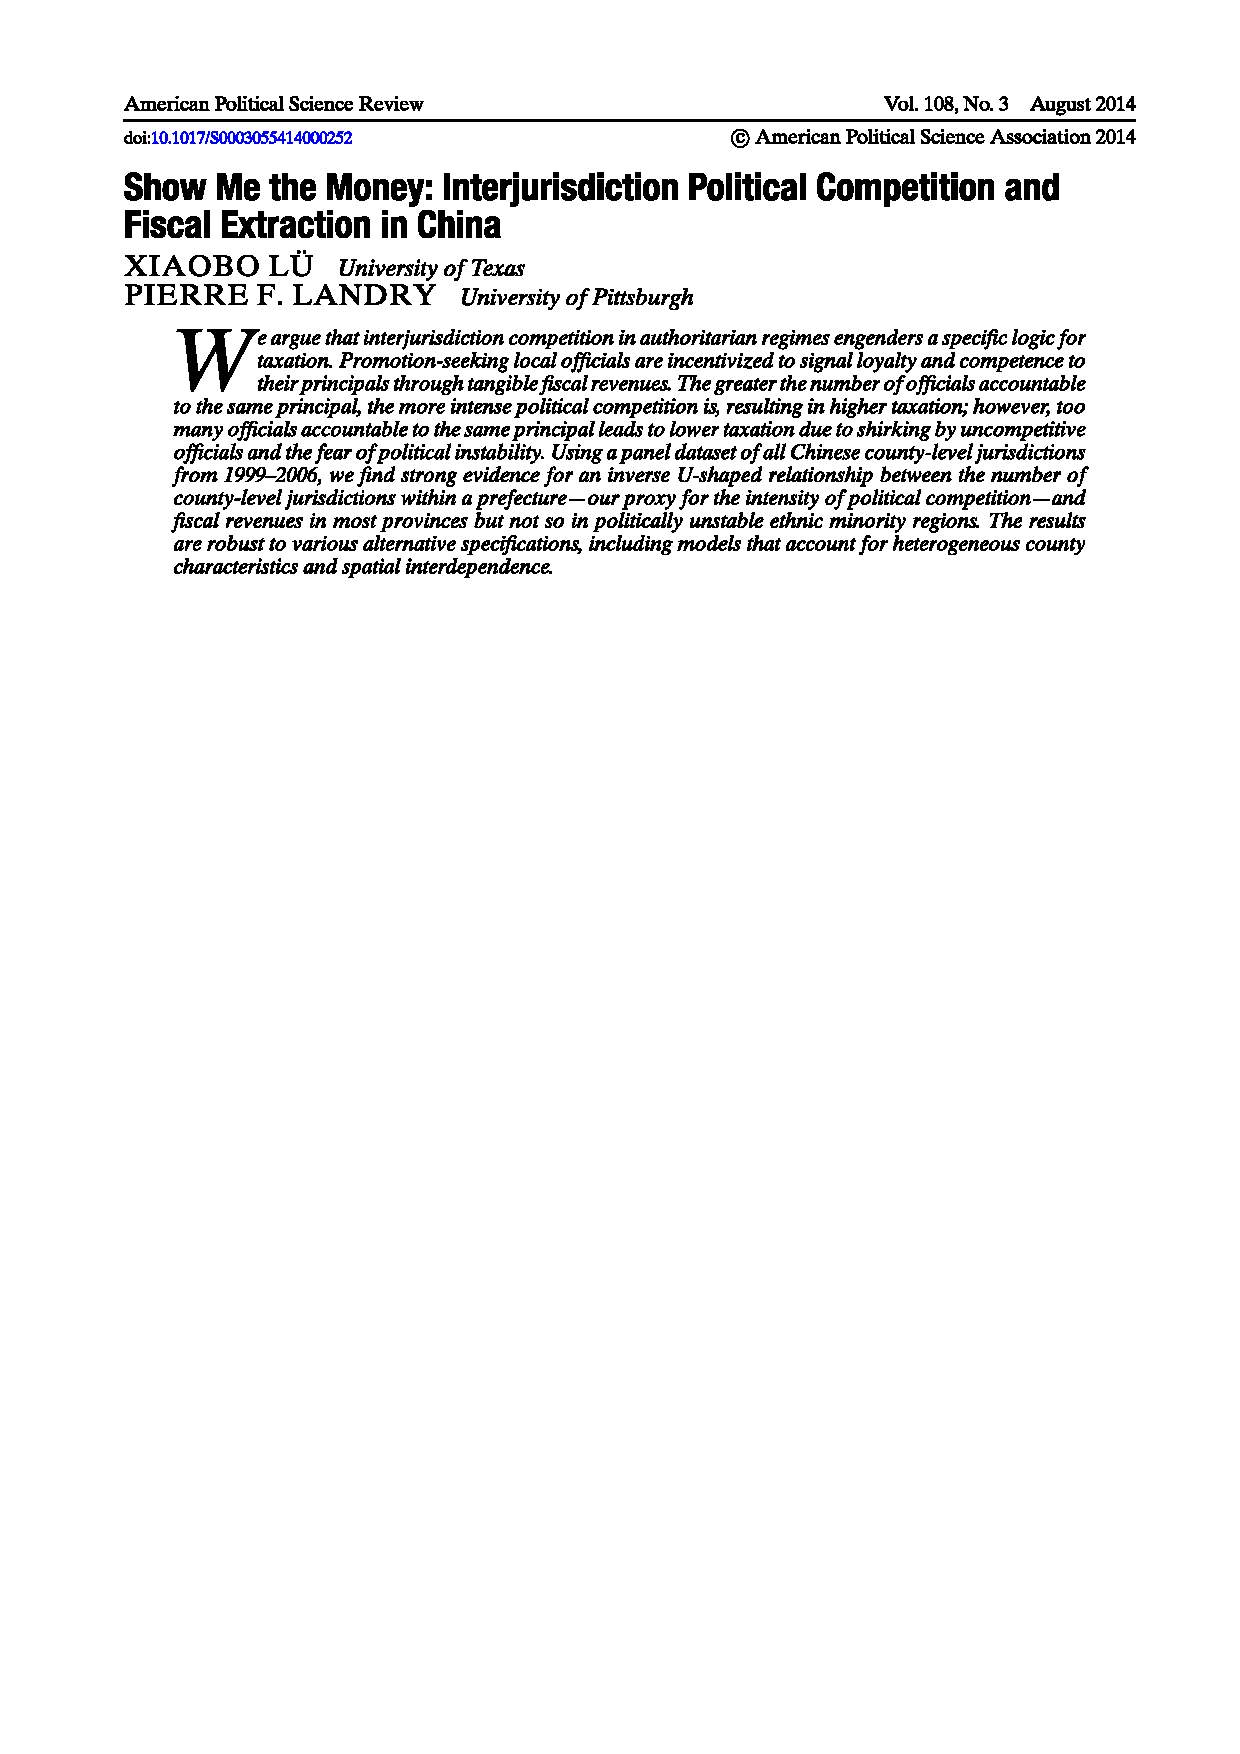
\includegraphics[width=0.9\linewidth]{Figs/Examples/lu_cover} \end{center}
\end{frame}

\begin{frame}
\begin{center}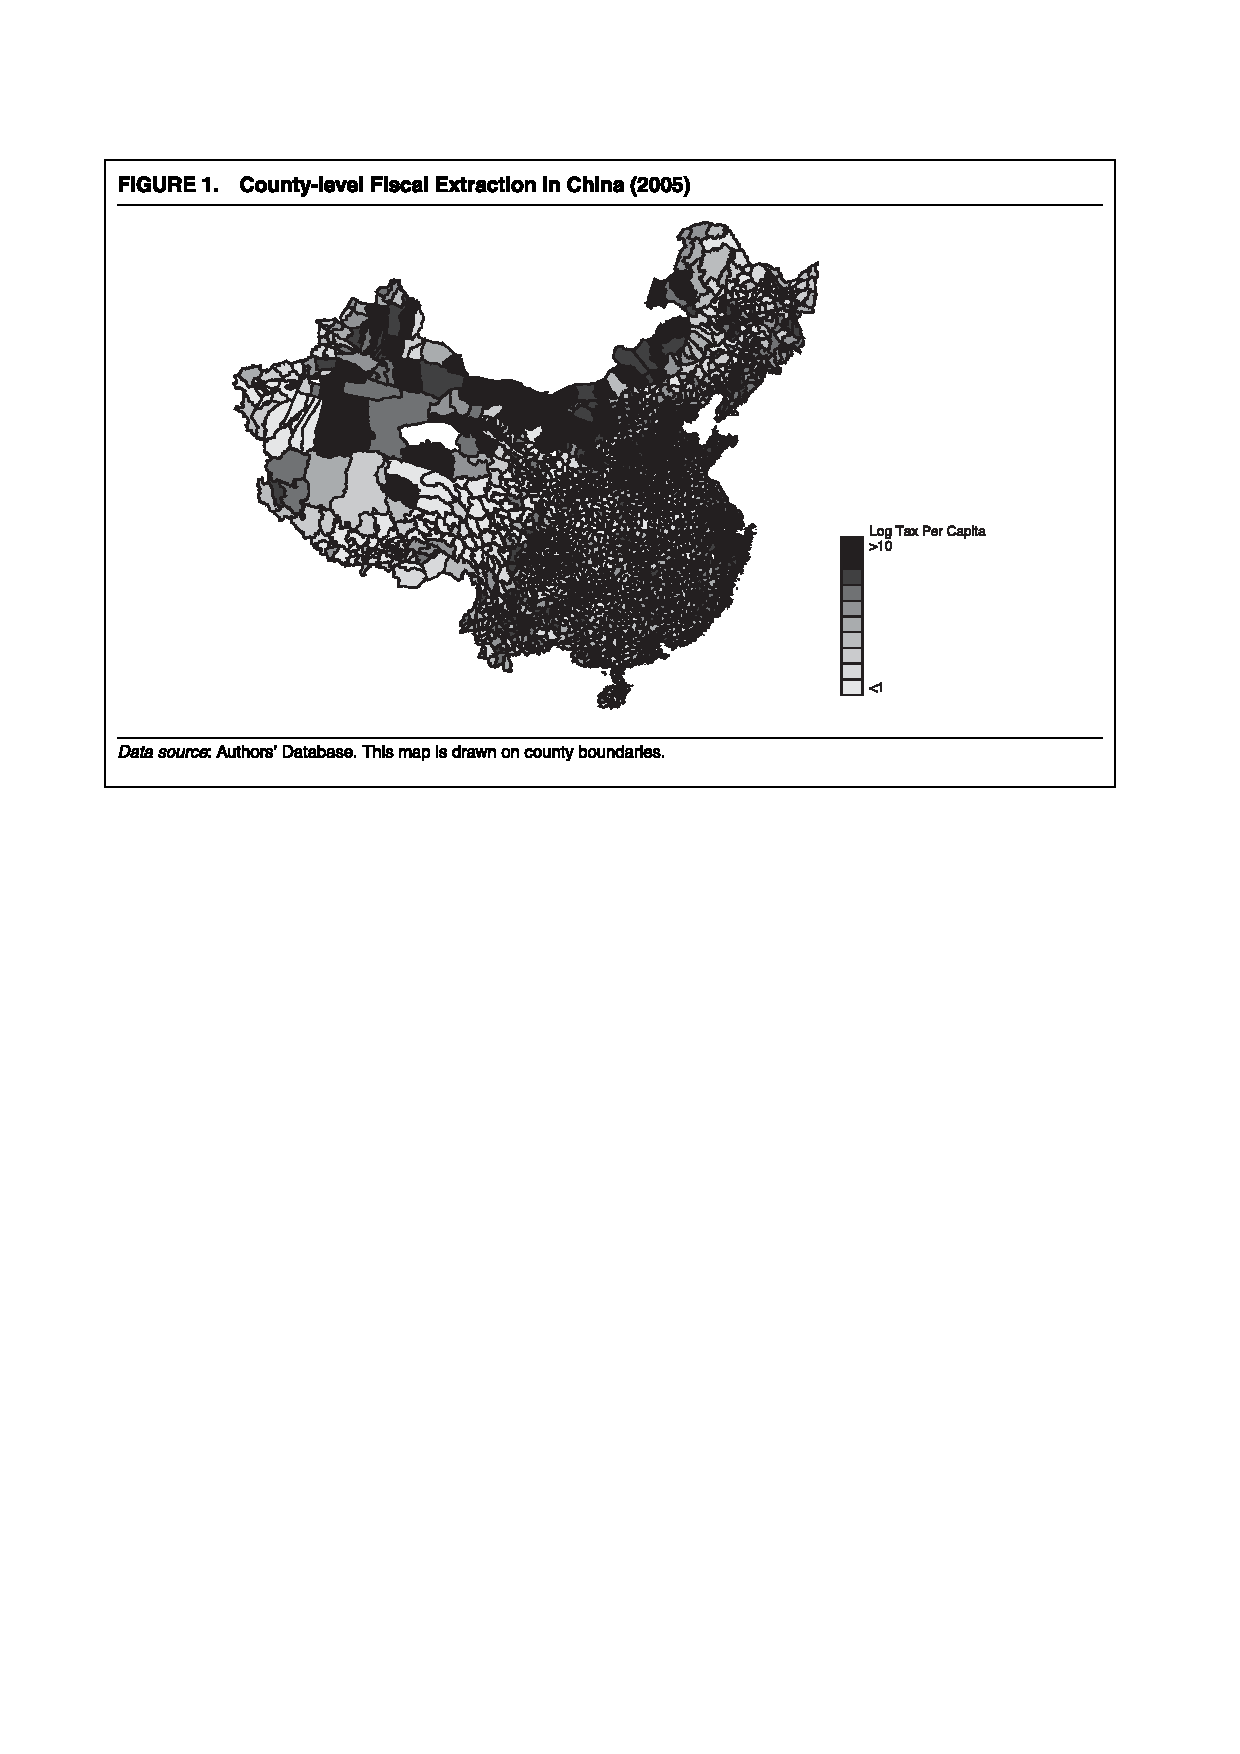
\includegraphics[width=0.9\linewidth]{Figs/Examples/lu_fig1} \end{center}
\end{frame}

\begin{frame}
\begin{center}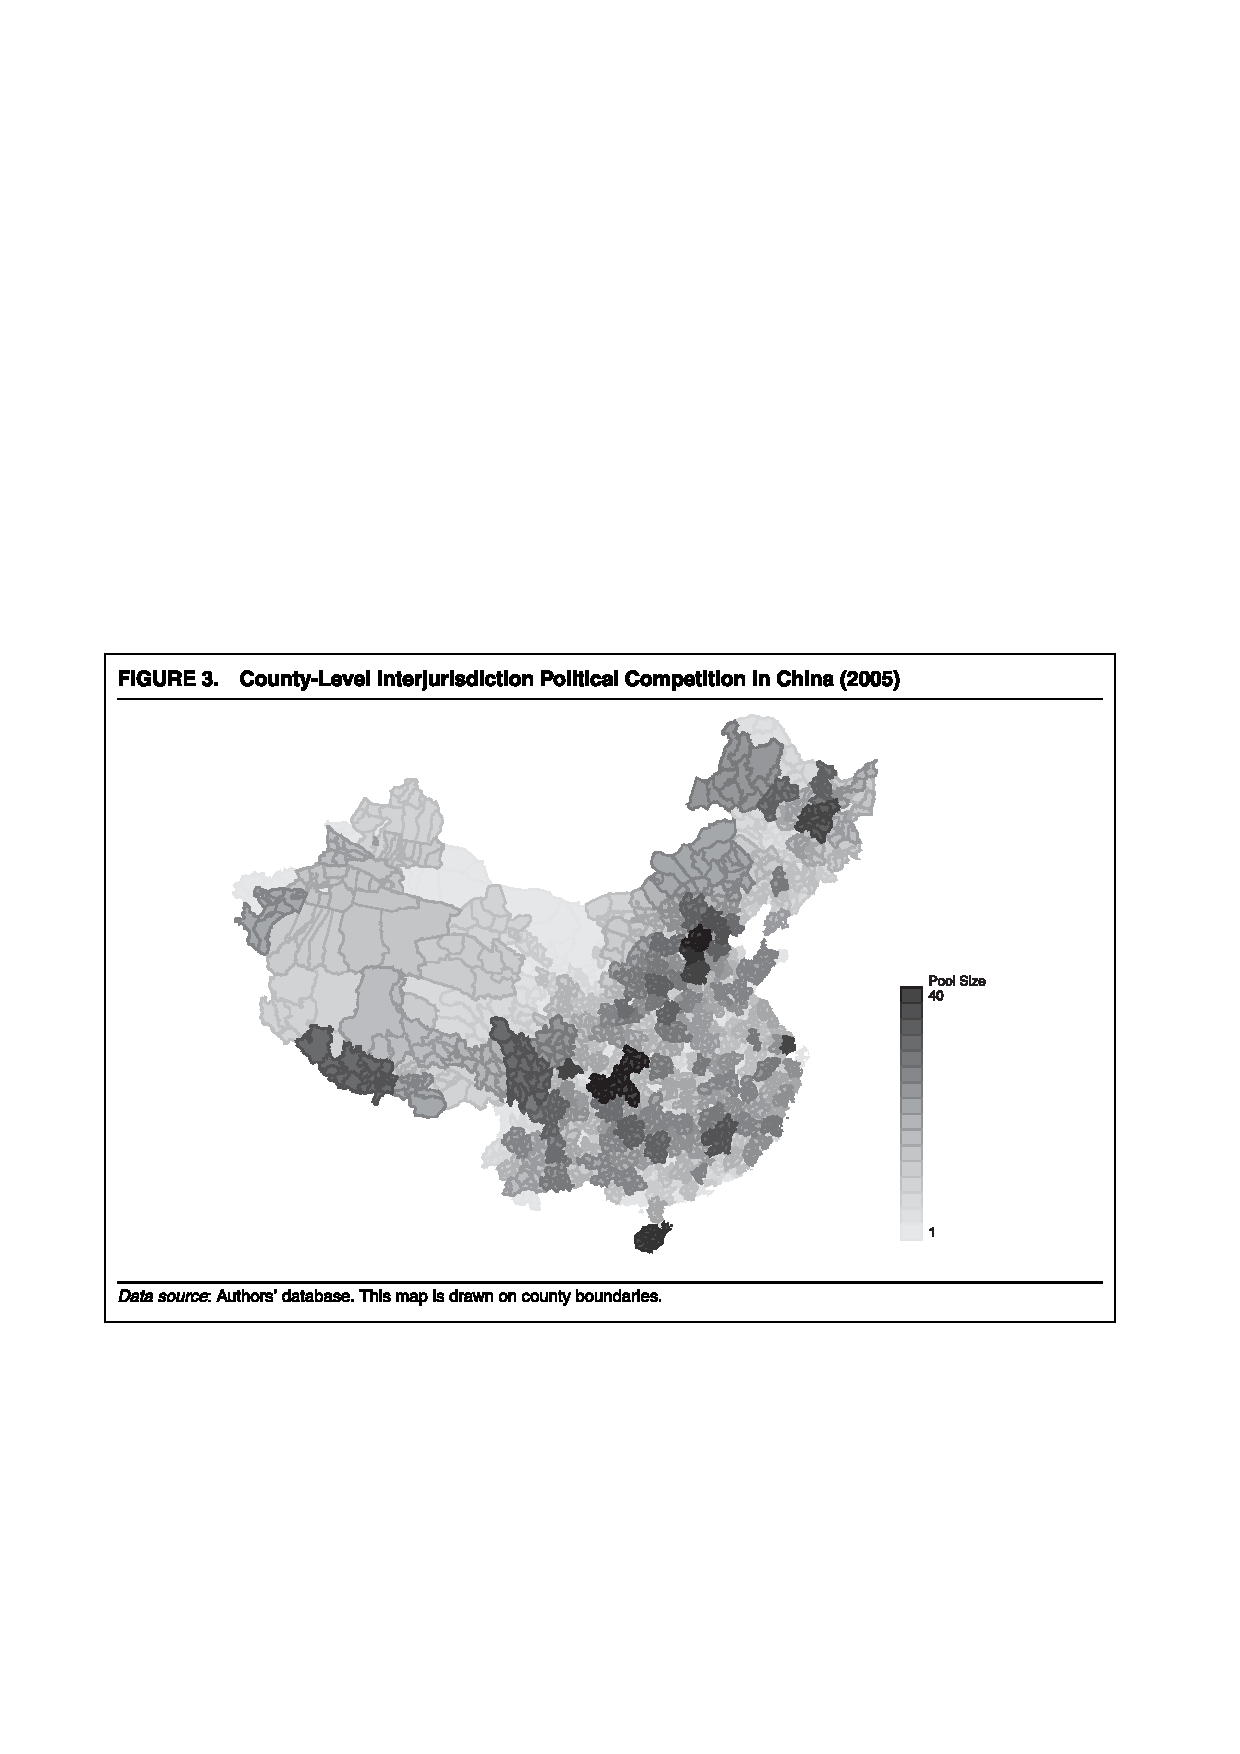
\includegraphics[width=0.9\linewidth]{Figs/Examples/lu_fig2} \end{center}
\end{frame}

\begin{frame}
\begin{center}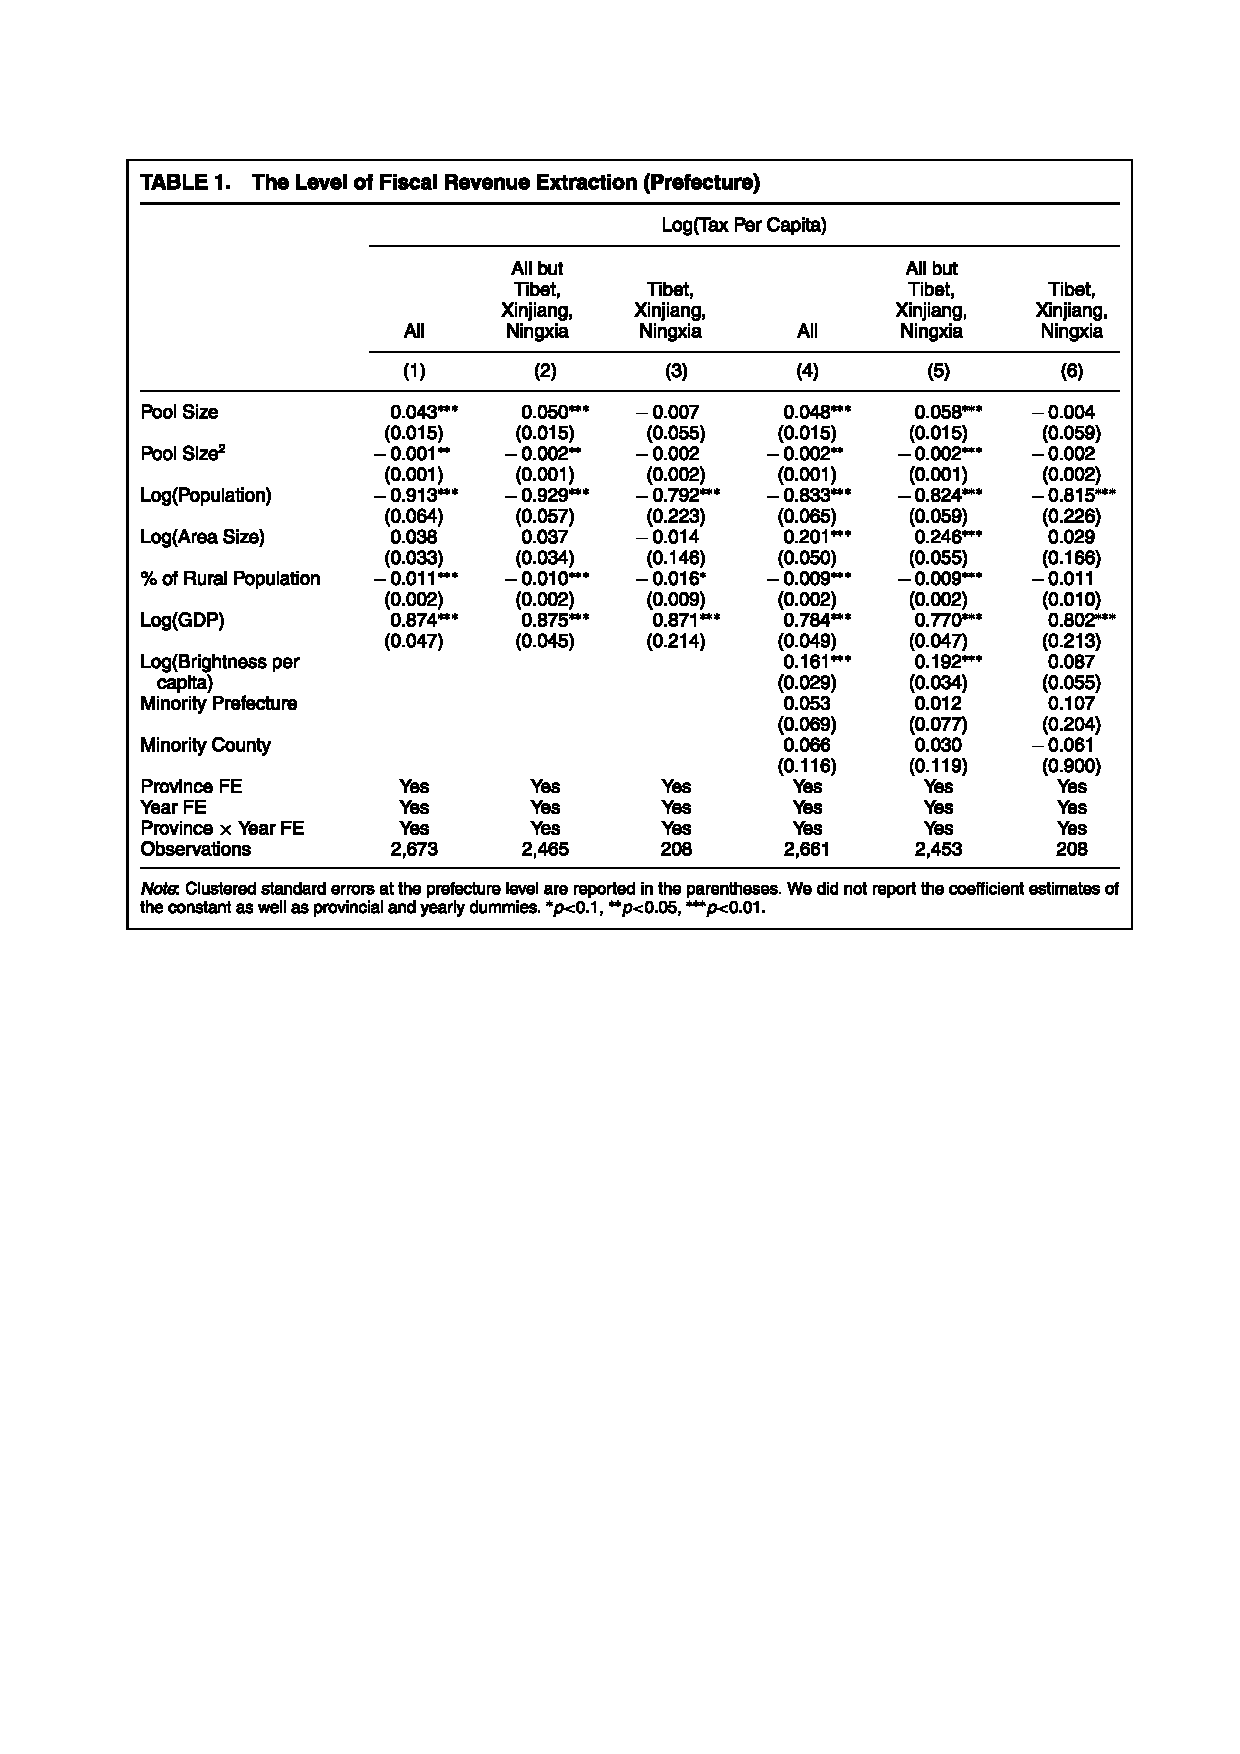
\includegraphics[width=0.9\linewidth]{Figs/Examples/lu_res} \end{center}
\end{frame}

\begin{frame}
\begin{center}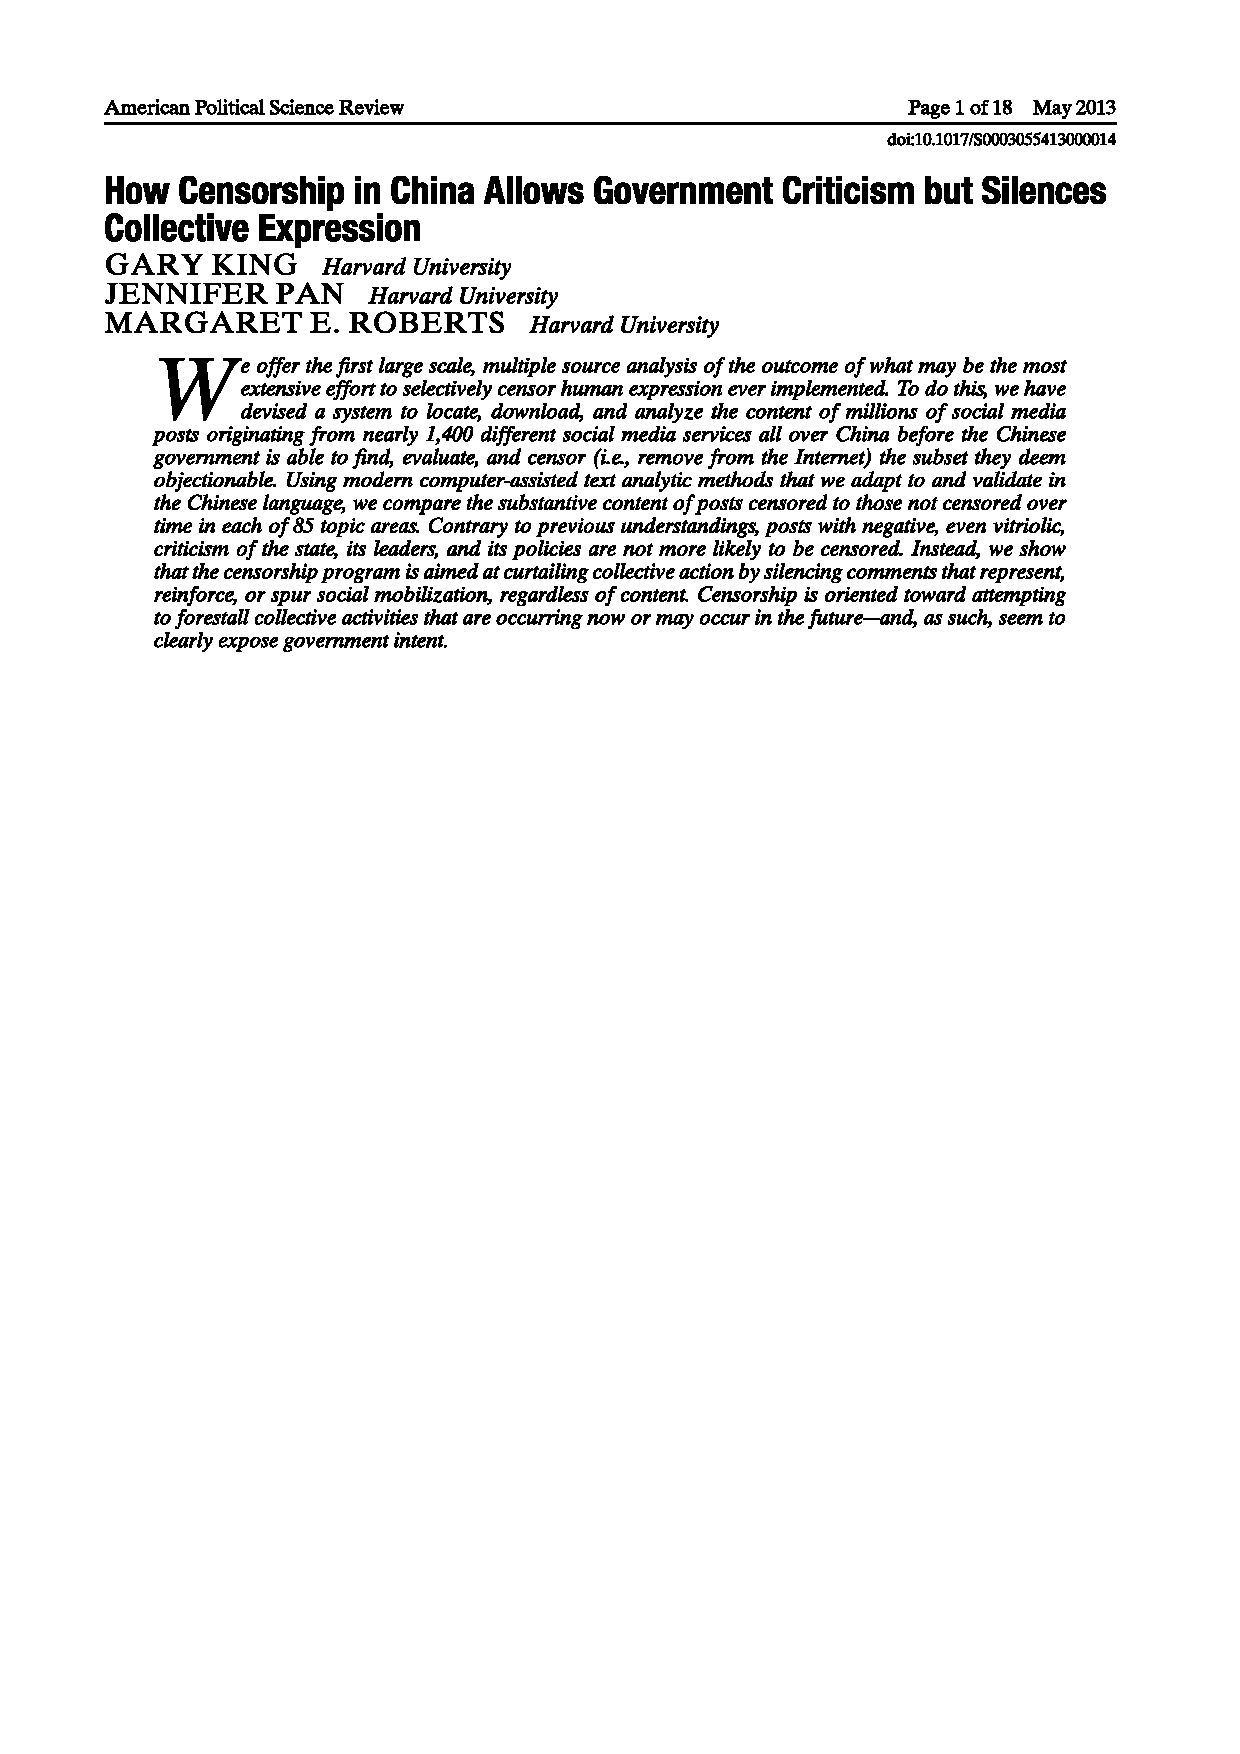
\includegraphics[width=0.9\linewidth]{Figs/Examples/molly_cover} \end{center}
\end{frame}

\begin{frame}
\begin{center}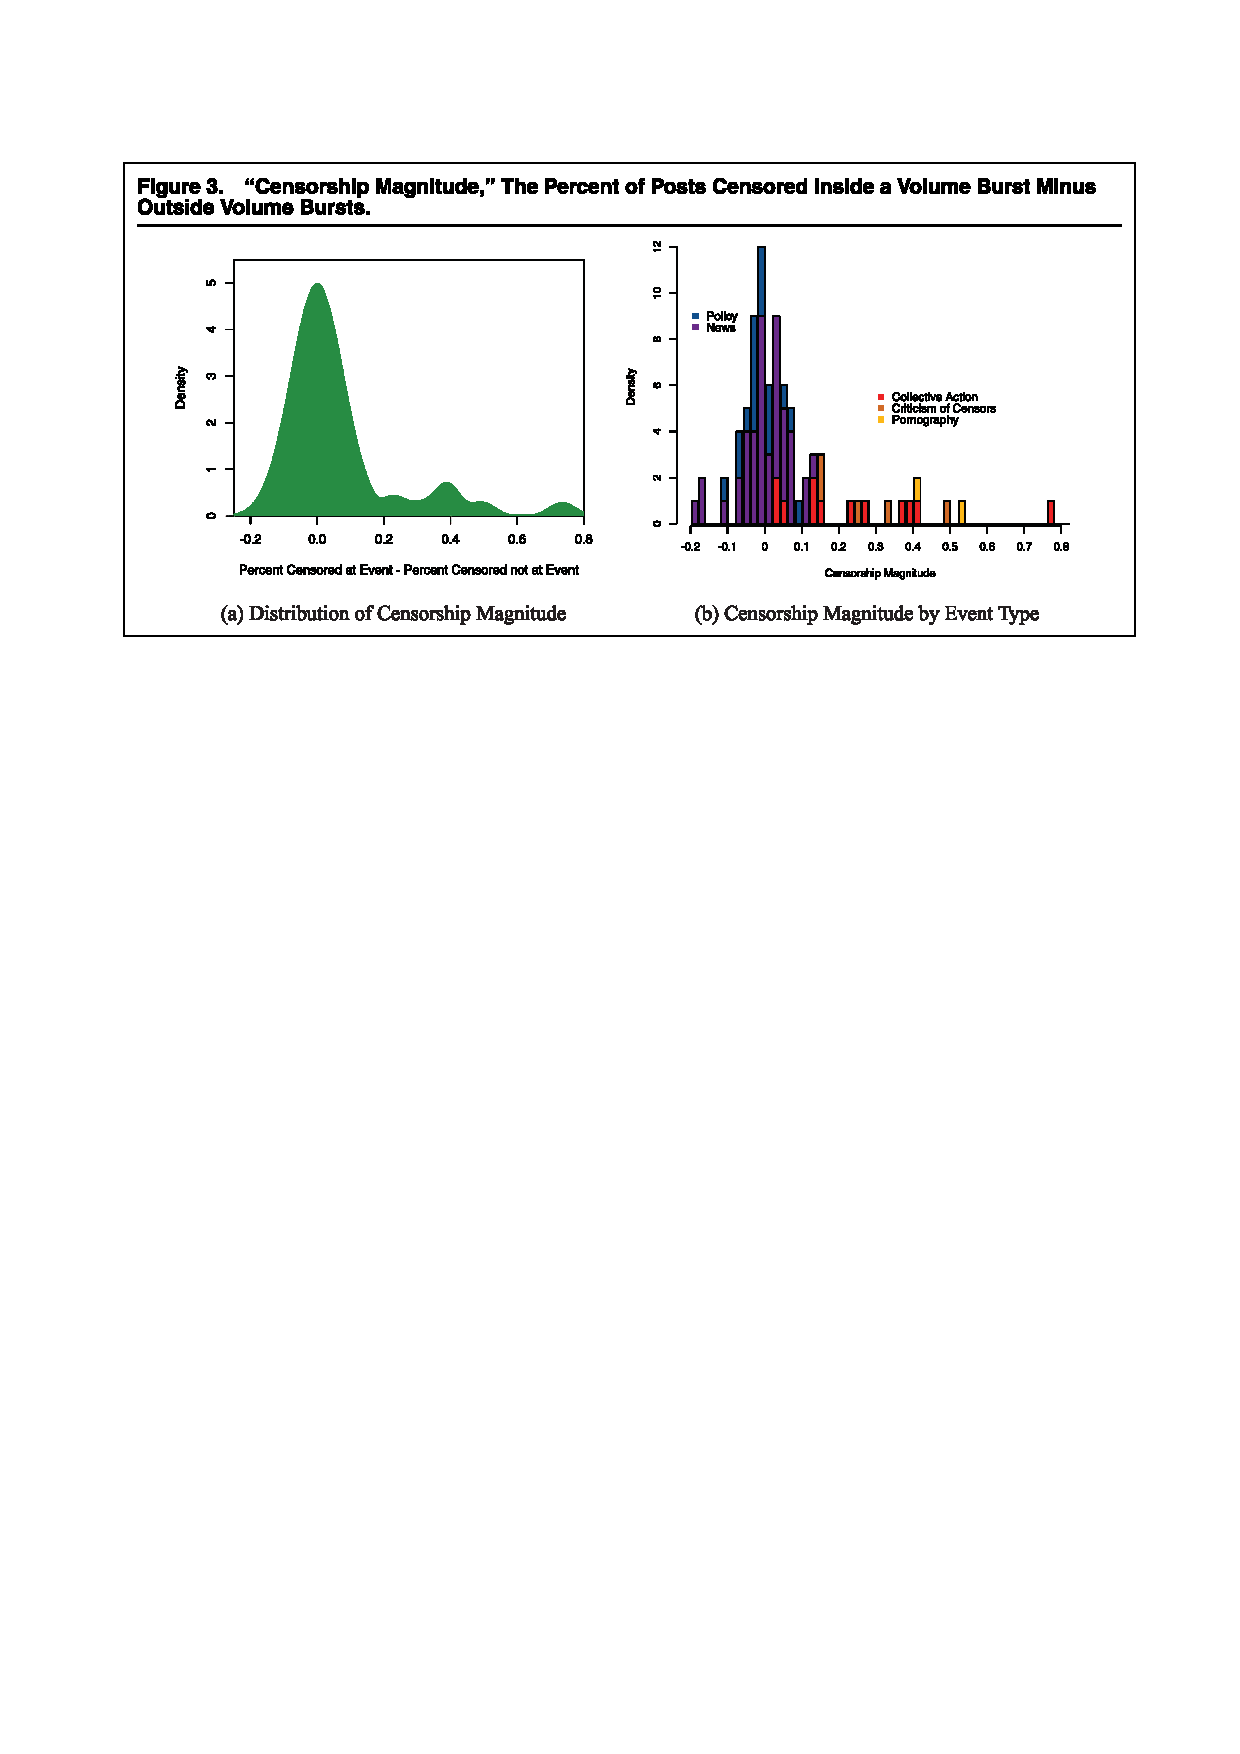
\includegraphics[width=0.9\linewidth]{Figs/Examples/molly_res} \end{center}
\end{frame}

\begin{frame}
\begin{center}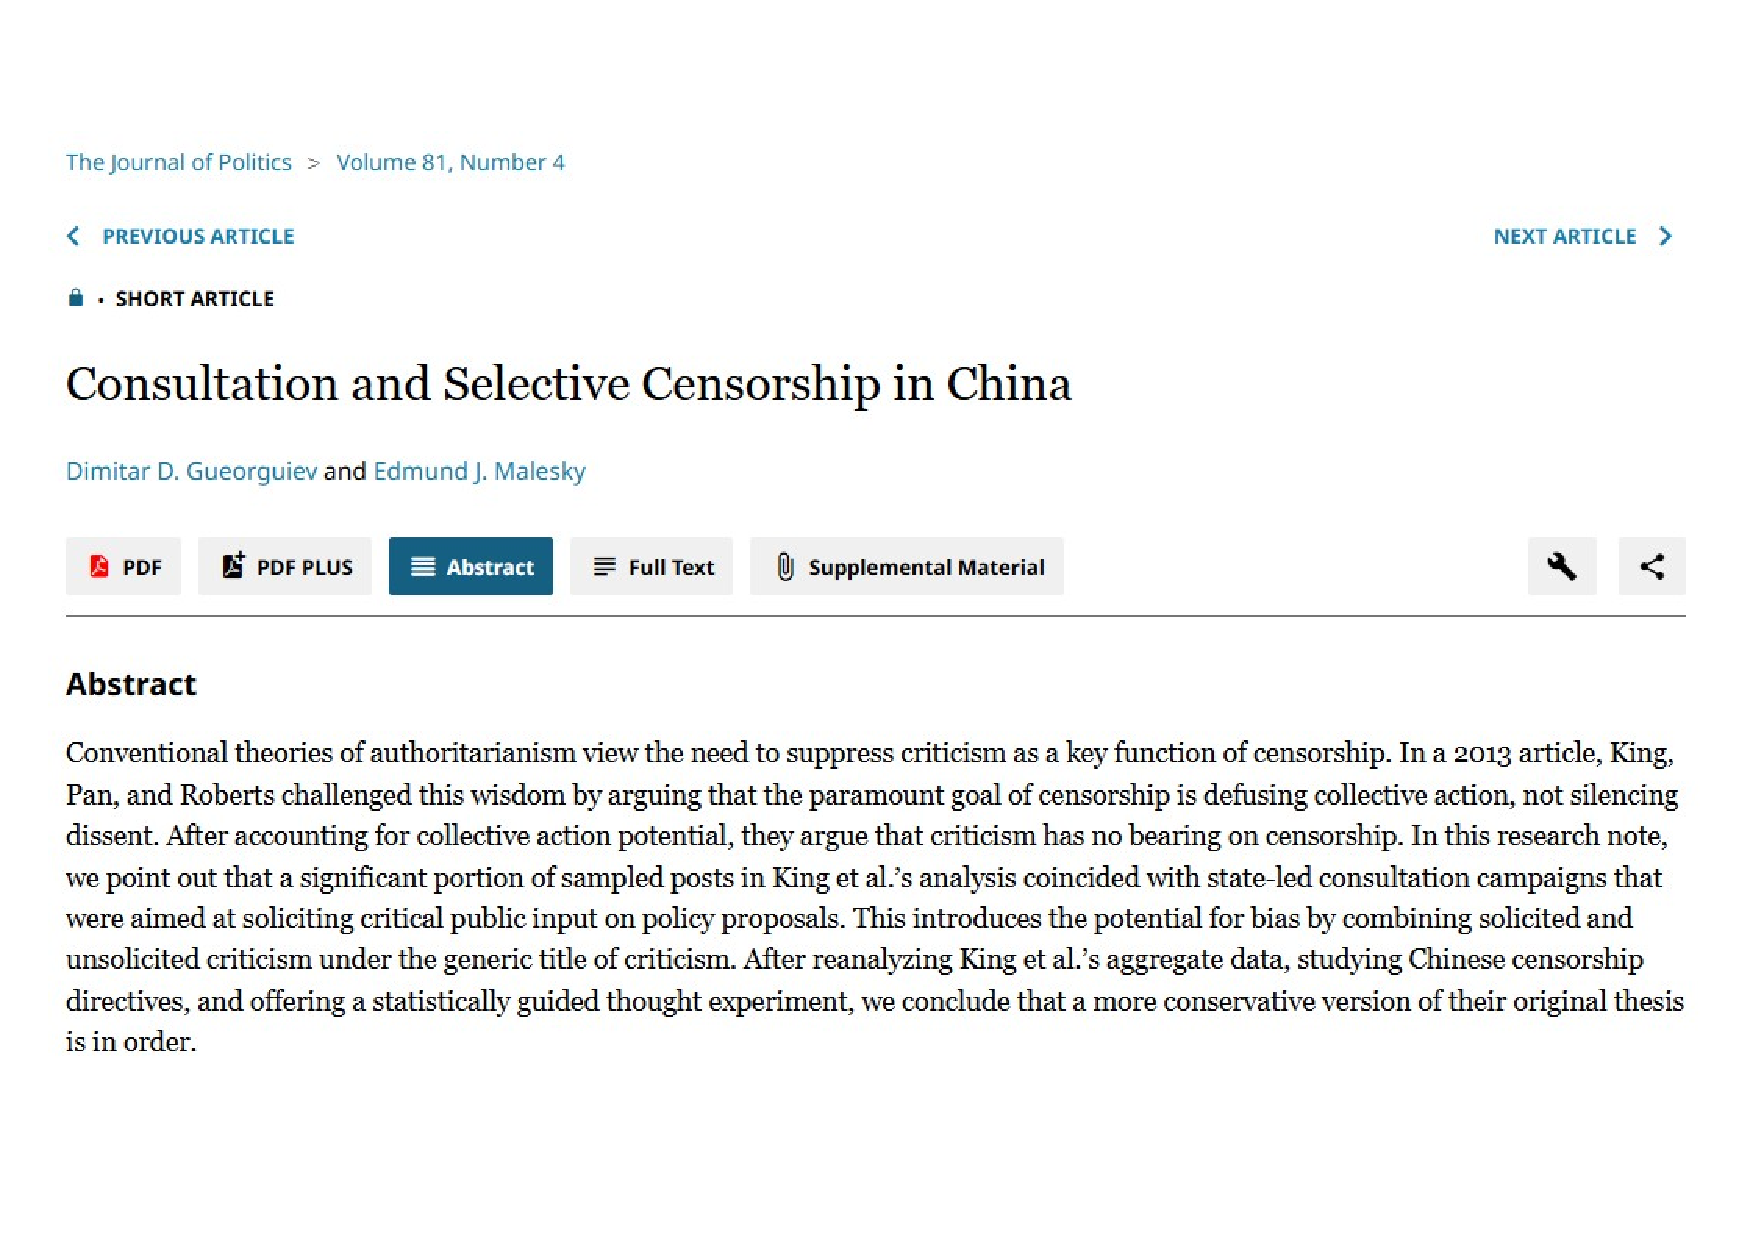
\includegraphics[width=0.9\linewidth]{Figs/Examples/molly_counter} \end{center}
\end{frame}

\begin{frame}
\begin{center}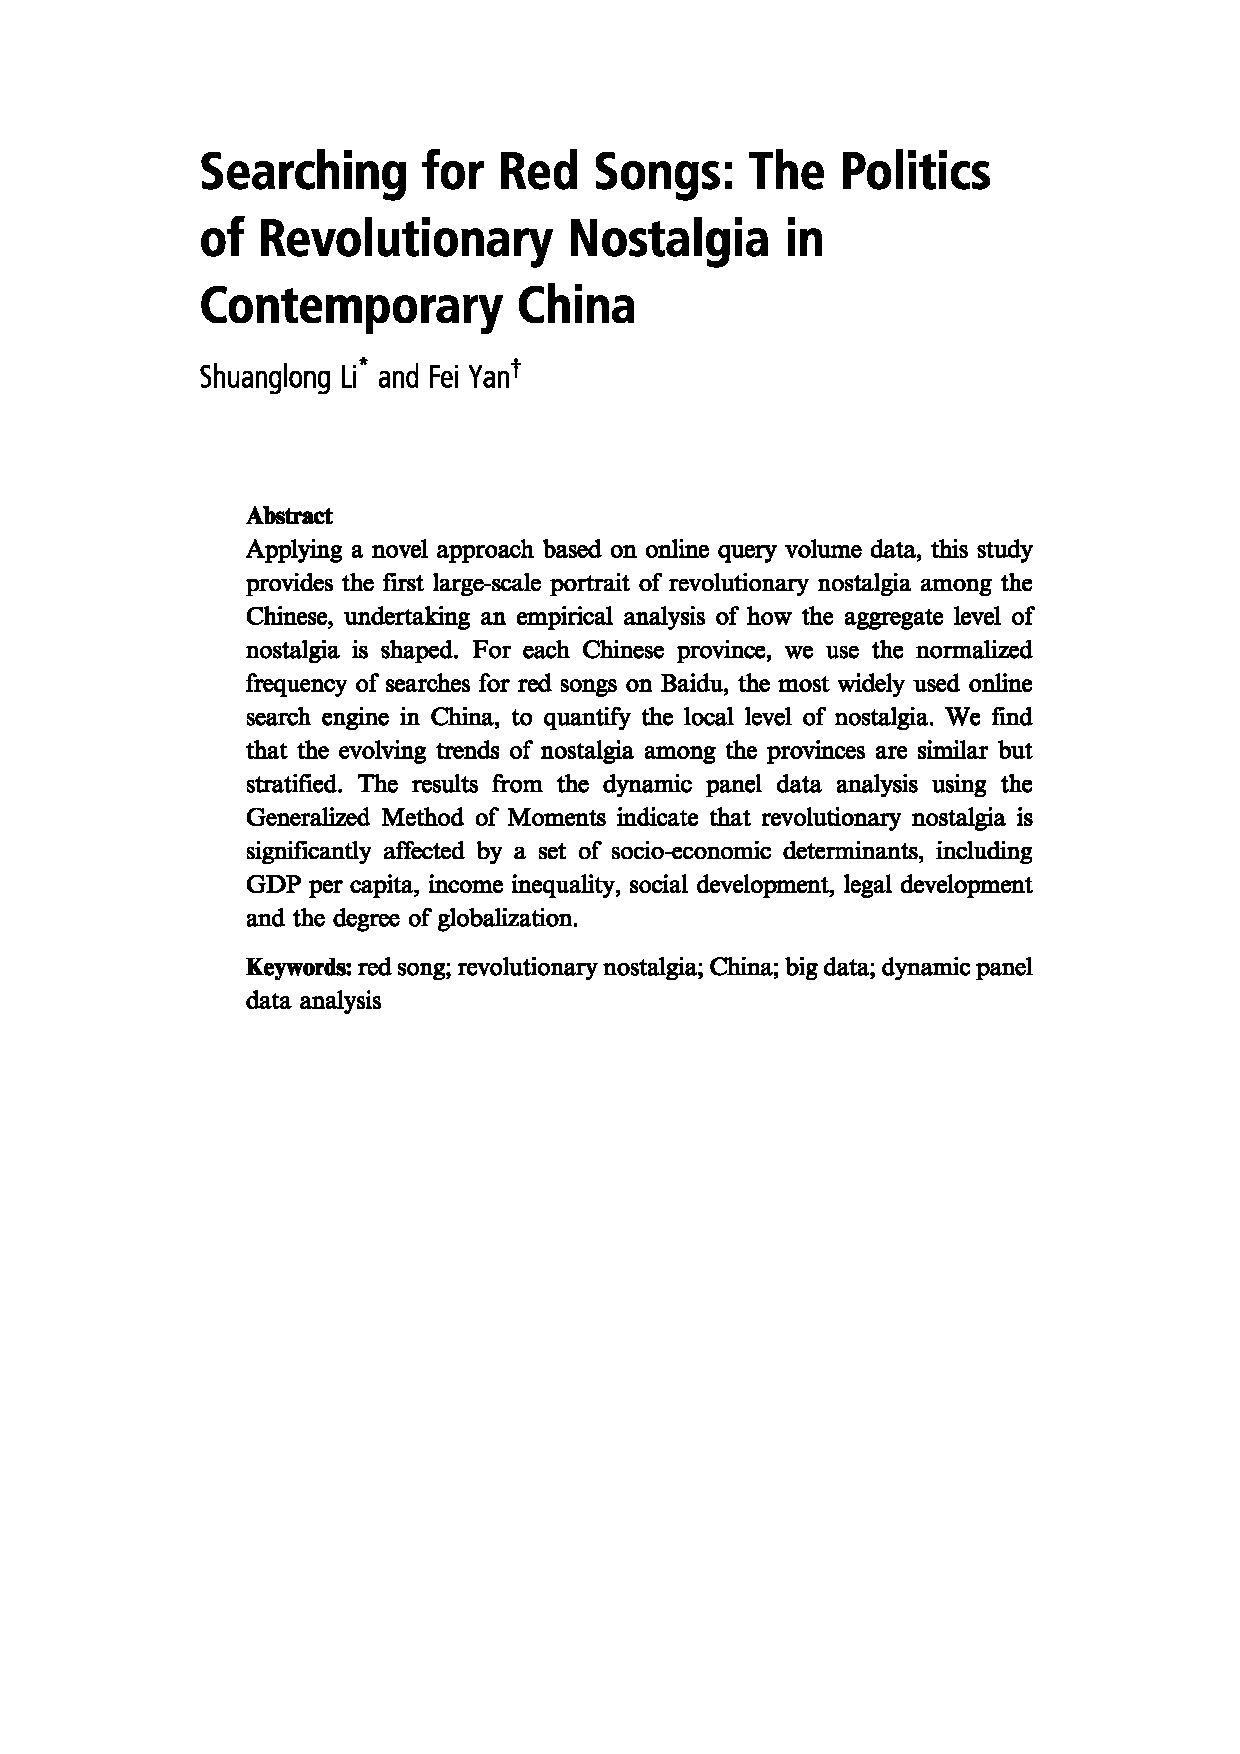
\includegraphics[width=0.8\linewidth]{Figs/Examples/yan_cover} \end{center}
\end{frame}

\begin{frame}
\begin{center}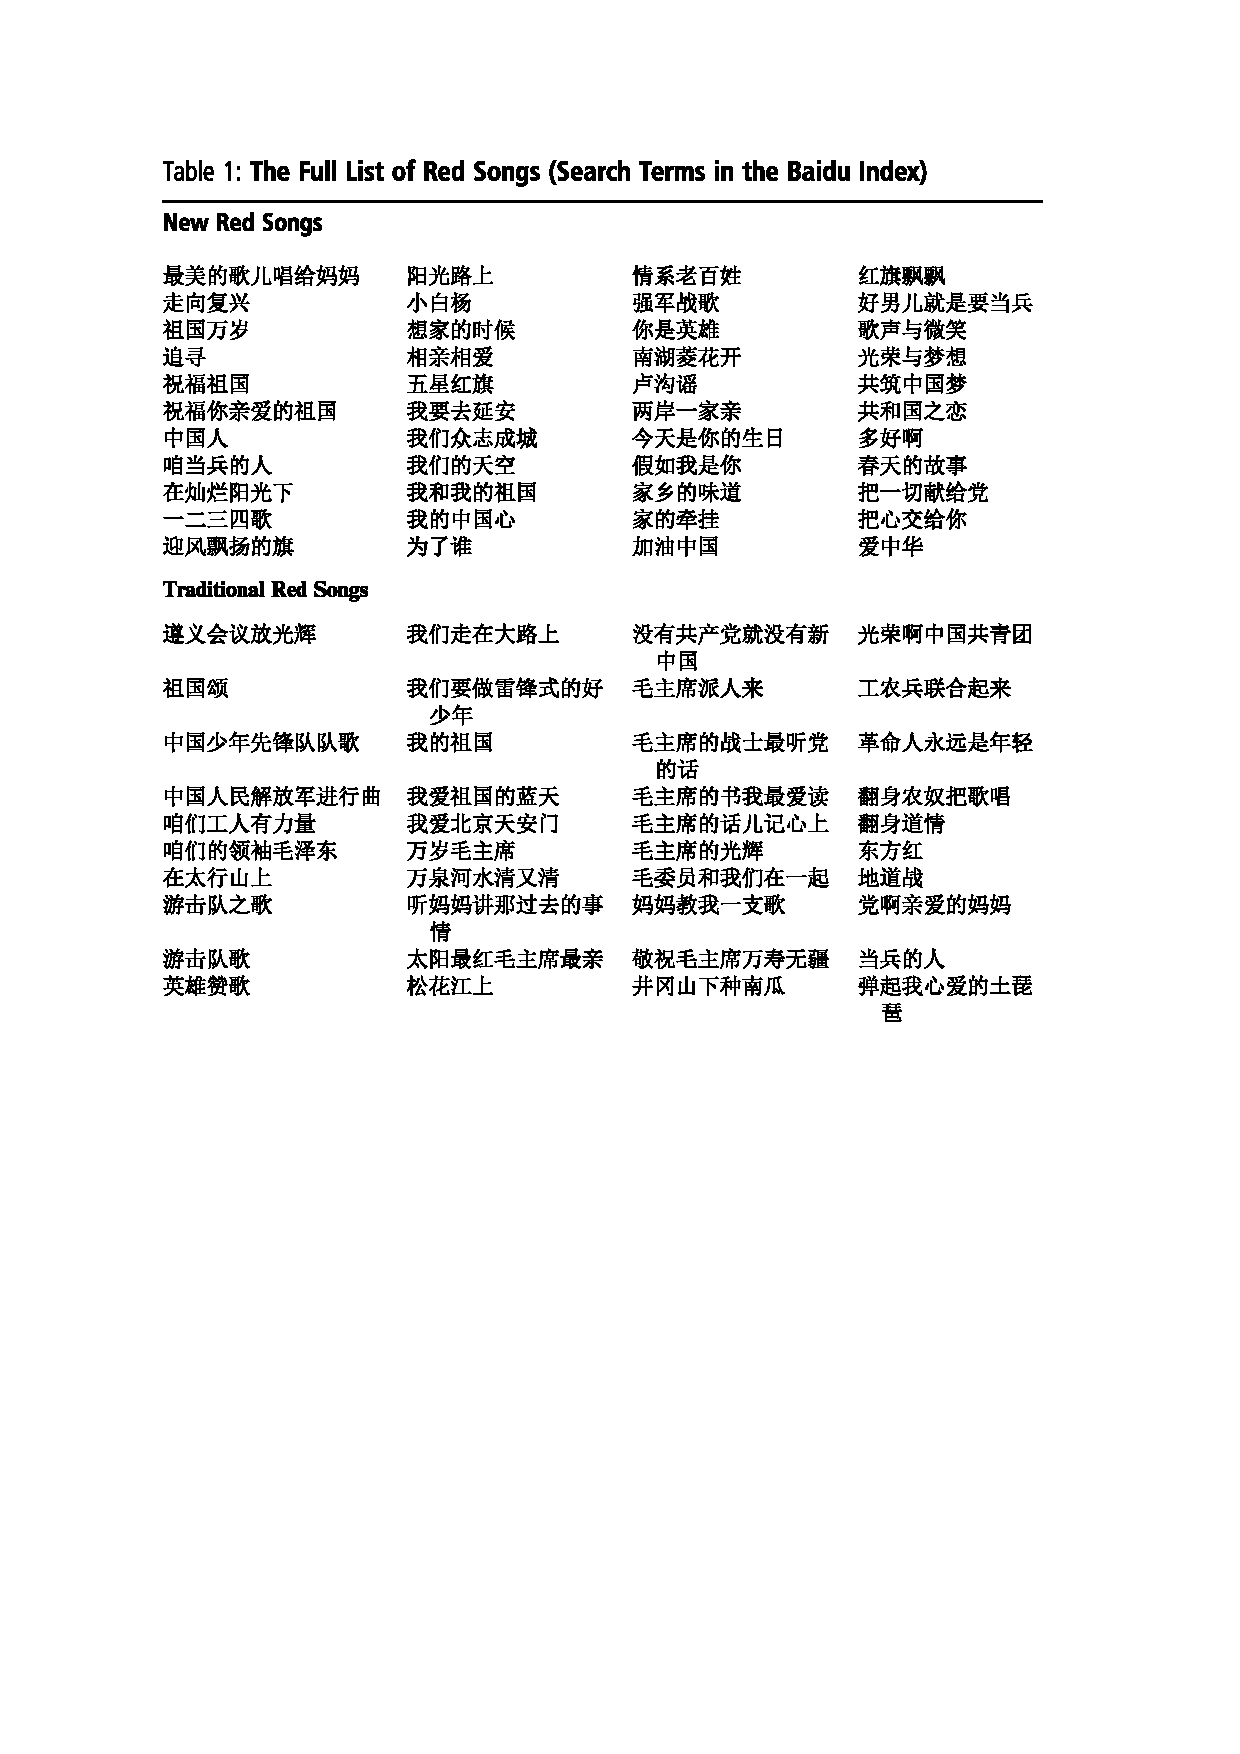
\includegraphics[width=0.9\linewidth]{Figs/Examples/yan_table} \end{center}
\end{frame}

\begin{frame}
\begin{center}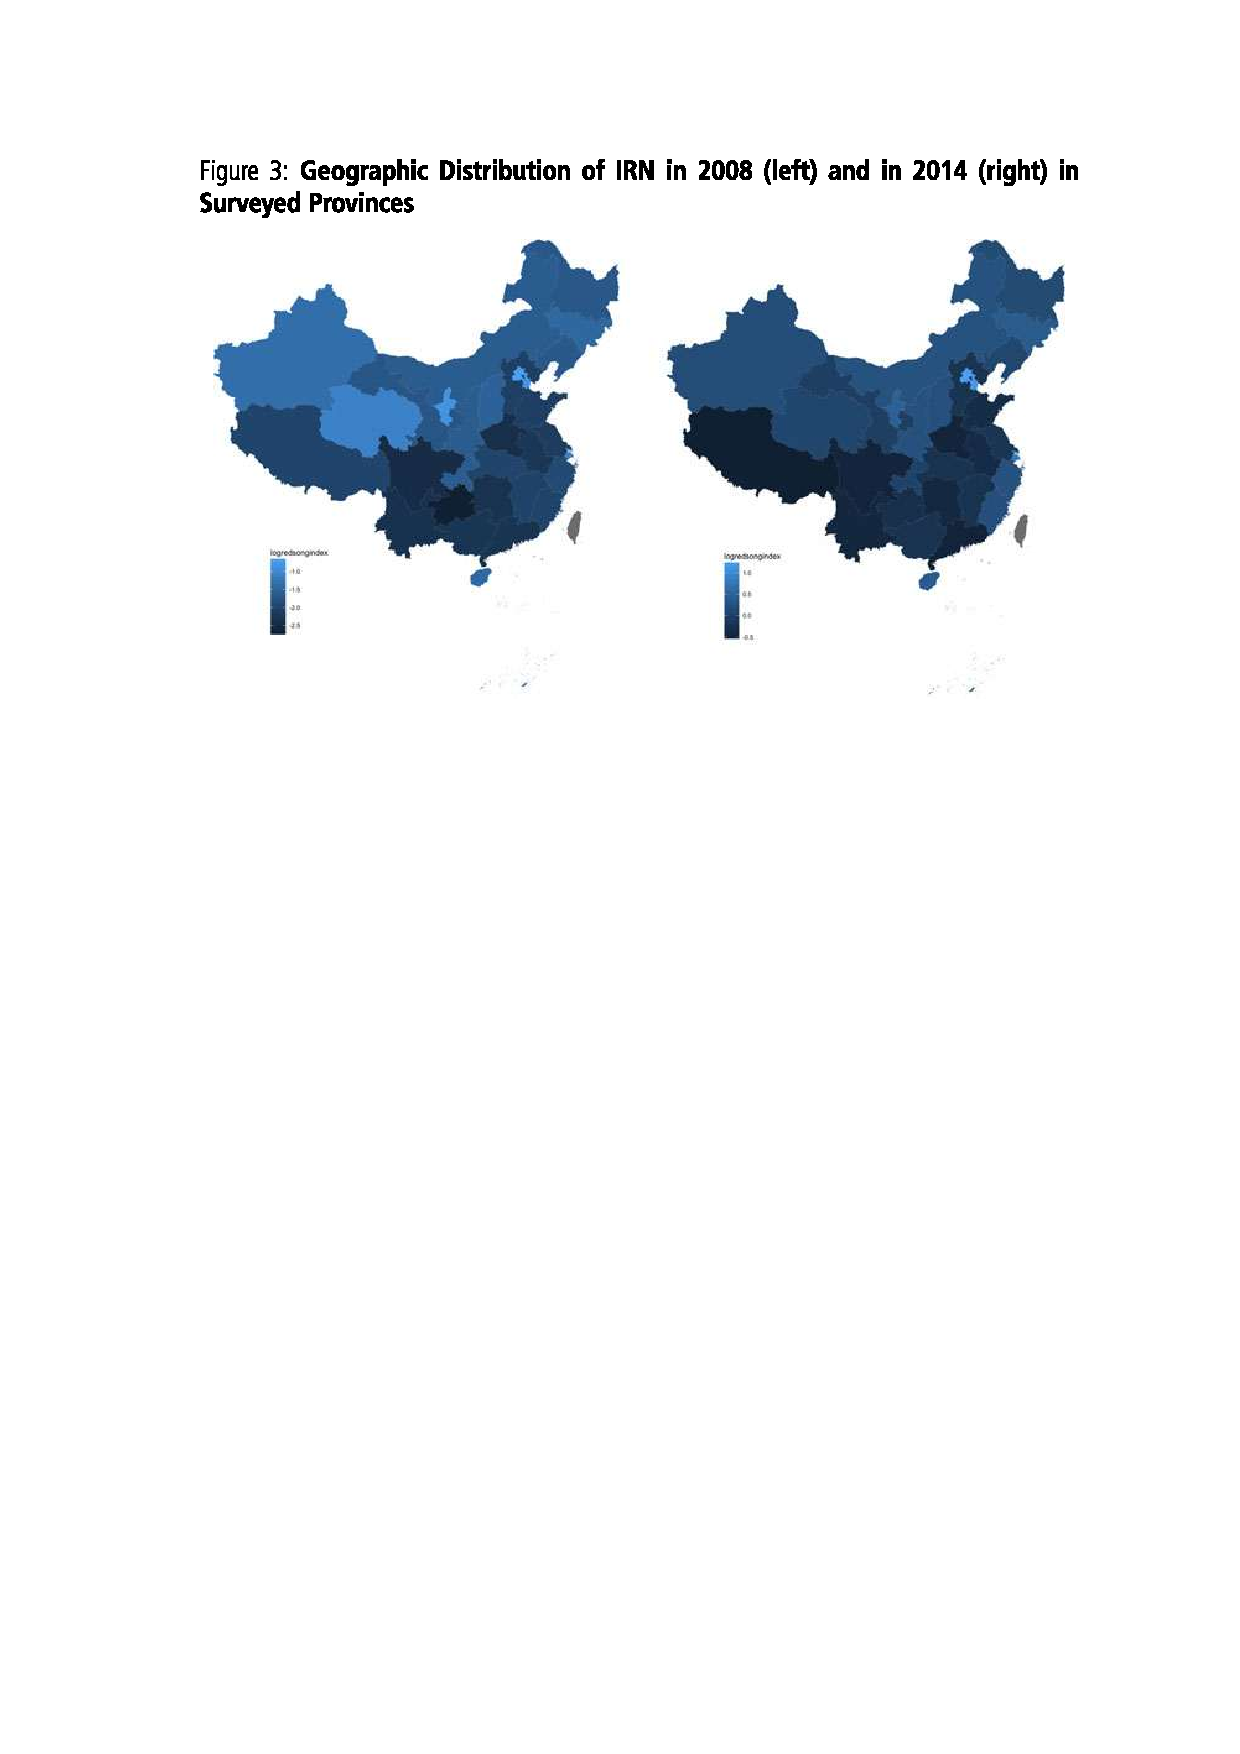
\includegraphics[width=0.9\linewidth]{Figs/Examples/yan_res} \end{center}
\end{frame}

\begin{frame}{Work with data}
\phantomsection\label{work-with-data}
\begin{itemize}
  \item Training for different \textbf{research methods}
  \vspace{1cm}
  \item A grasp of potential \textbf{data sources}
  \vspace{1cm}
  \item Solid and deep \textbf{field experiences} and/or \textbf{subject knowledge}
\end{itemize}
\end{frame}

\begin{frame}
\begin{itemize}
  \item Training for different \textbf{research methods}
  \vspace{0.1cm}
  \begin{itemize}
    \item Qualitative: Case study (Bayesian and machine learning), ethnography and (elite) interviews
    \item Quantitative: Econometrics and regression (frequentist and Bayesian), experiments and causal inference
    \item Computational: Text-as-data, social network analysis, geographic data science and ChatGPT-assisted research
  \end{itemize}
  \vspace{0.6cm}
  \item A grasp of potential \textbf{data sources}
  \vspace{0.6cm}
  \item Solid and deep \textbf{field experiences} and/or \textbf{subject knowledge}
\end{itemize}
\end{frame}

\begin{frame}
\begin{itemize}
  \item Training for different \textbf{research methods}
  \vspace{0.6cm}
  \item A grasp of potential \textbf{data sources}
  \vspace{0.1cm}
  \begin{itemize}
    \item Databases
    \item Libraries and archives
    \item Survey firms and research centres
    \item API and web scraping (i.e., coding and programming)
    \item Replication packs
  \end{itemize}
  \vspace{0.6cm}
  \item Solid and deep \textbf{field experiences} and/or \textbf{subject knowledge}
\end{itemize}
\end{frame}

\begin{frame}
\begin{itemize}
  \item Training for different \textbf{research methods}
  \vspace{1cm}
  \item A grasp of potential \textbf{data sources}
  \vspace{1cm}
  \item Solid and deep \textbf{field experiences} (e.g., politics of data generation and release) and/or \textbf{subject knowledge} (e.g., political selection and government finances)
\end{itemize}
\end{frame}

\begin{frame}{Data generation process is a political question}
\phantomsection\label{data-generation-process-is-a-political-question}
\begin{center}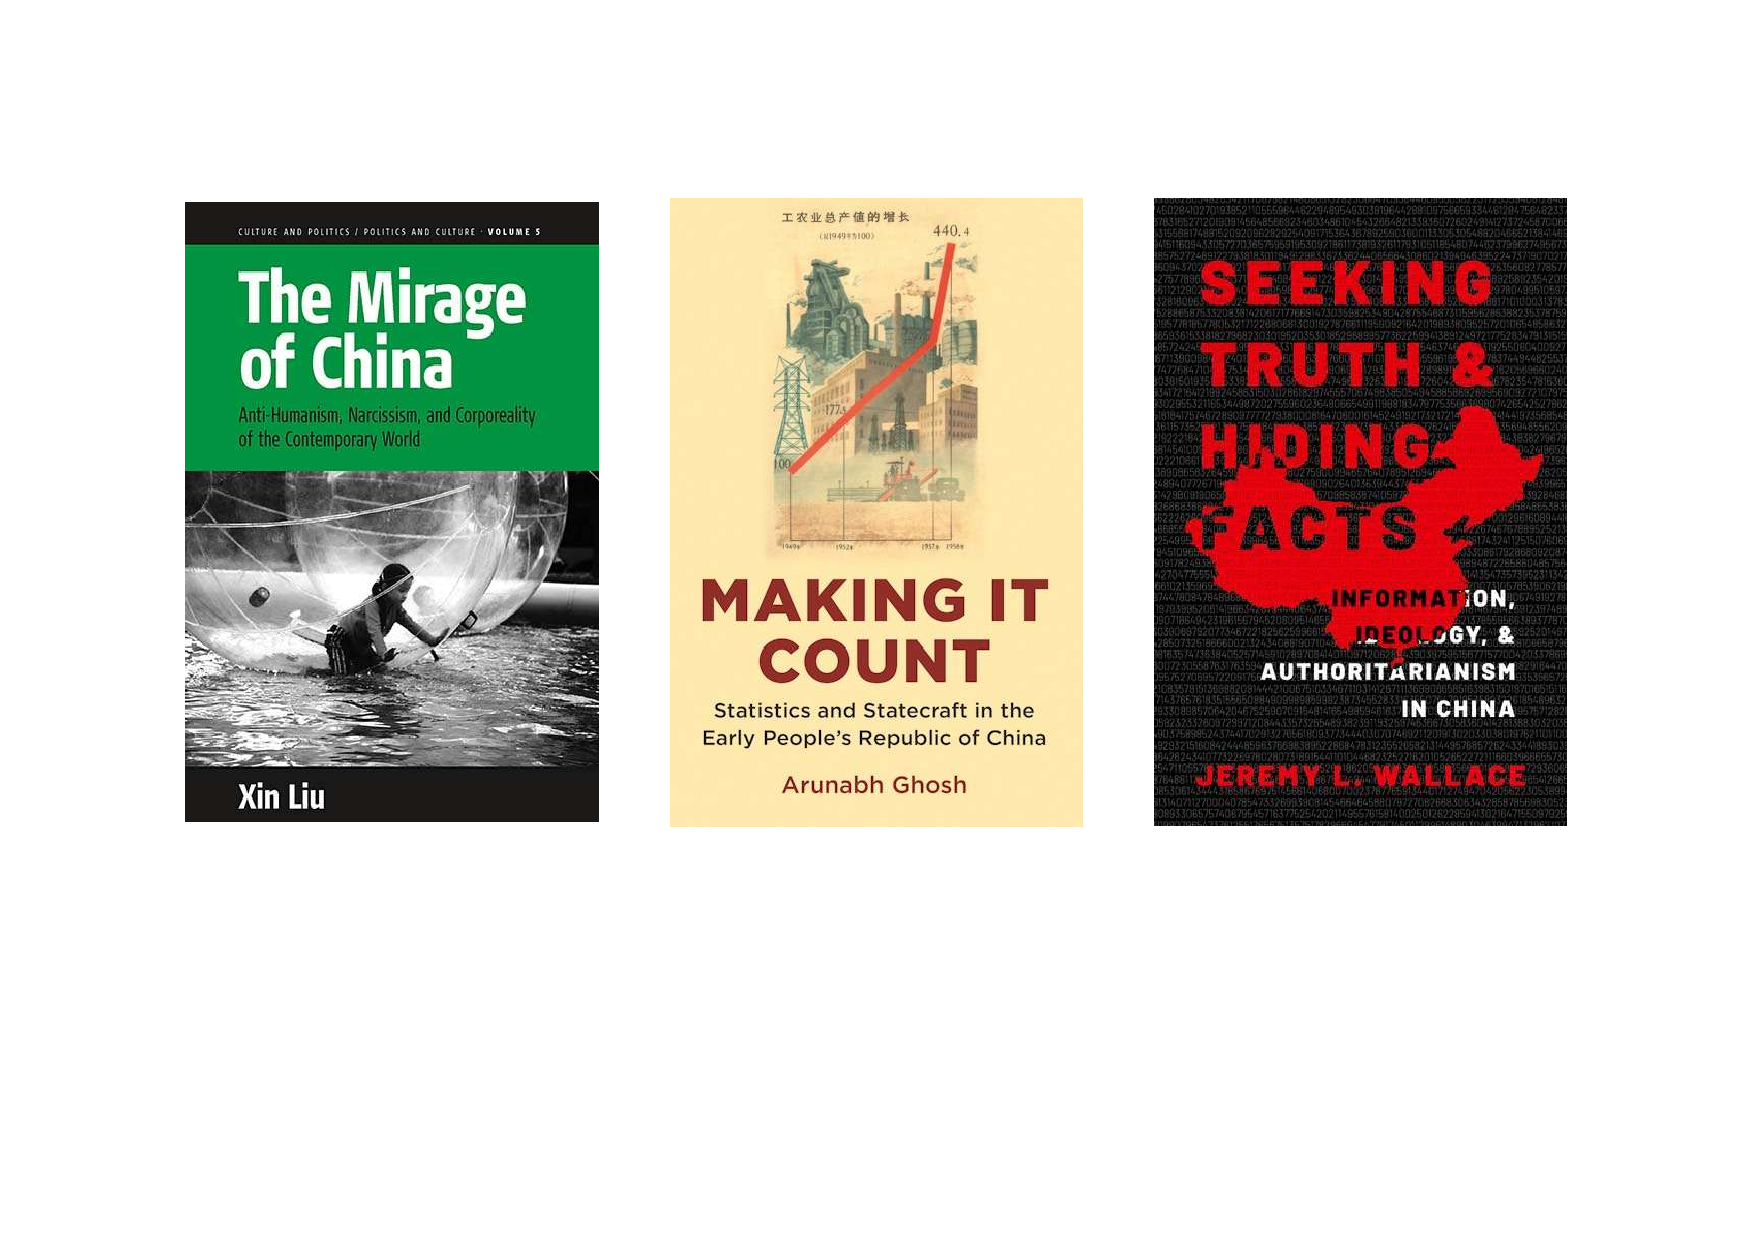
\includegraphics[width=1\linewidth]{Figs/books} \end{center}
\end{frame}

\begin{frame}
\begin{center}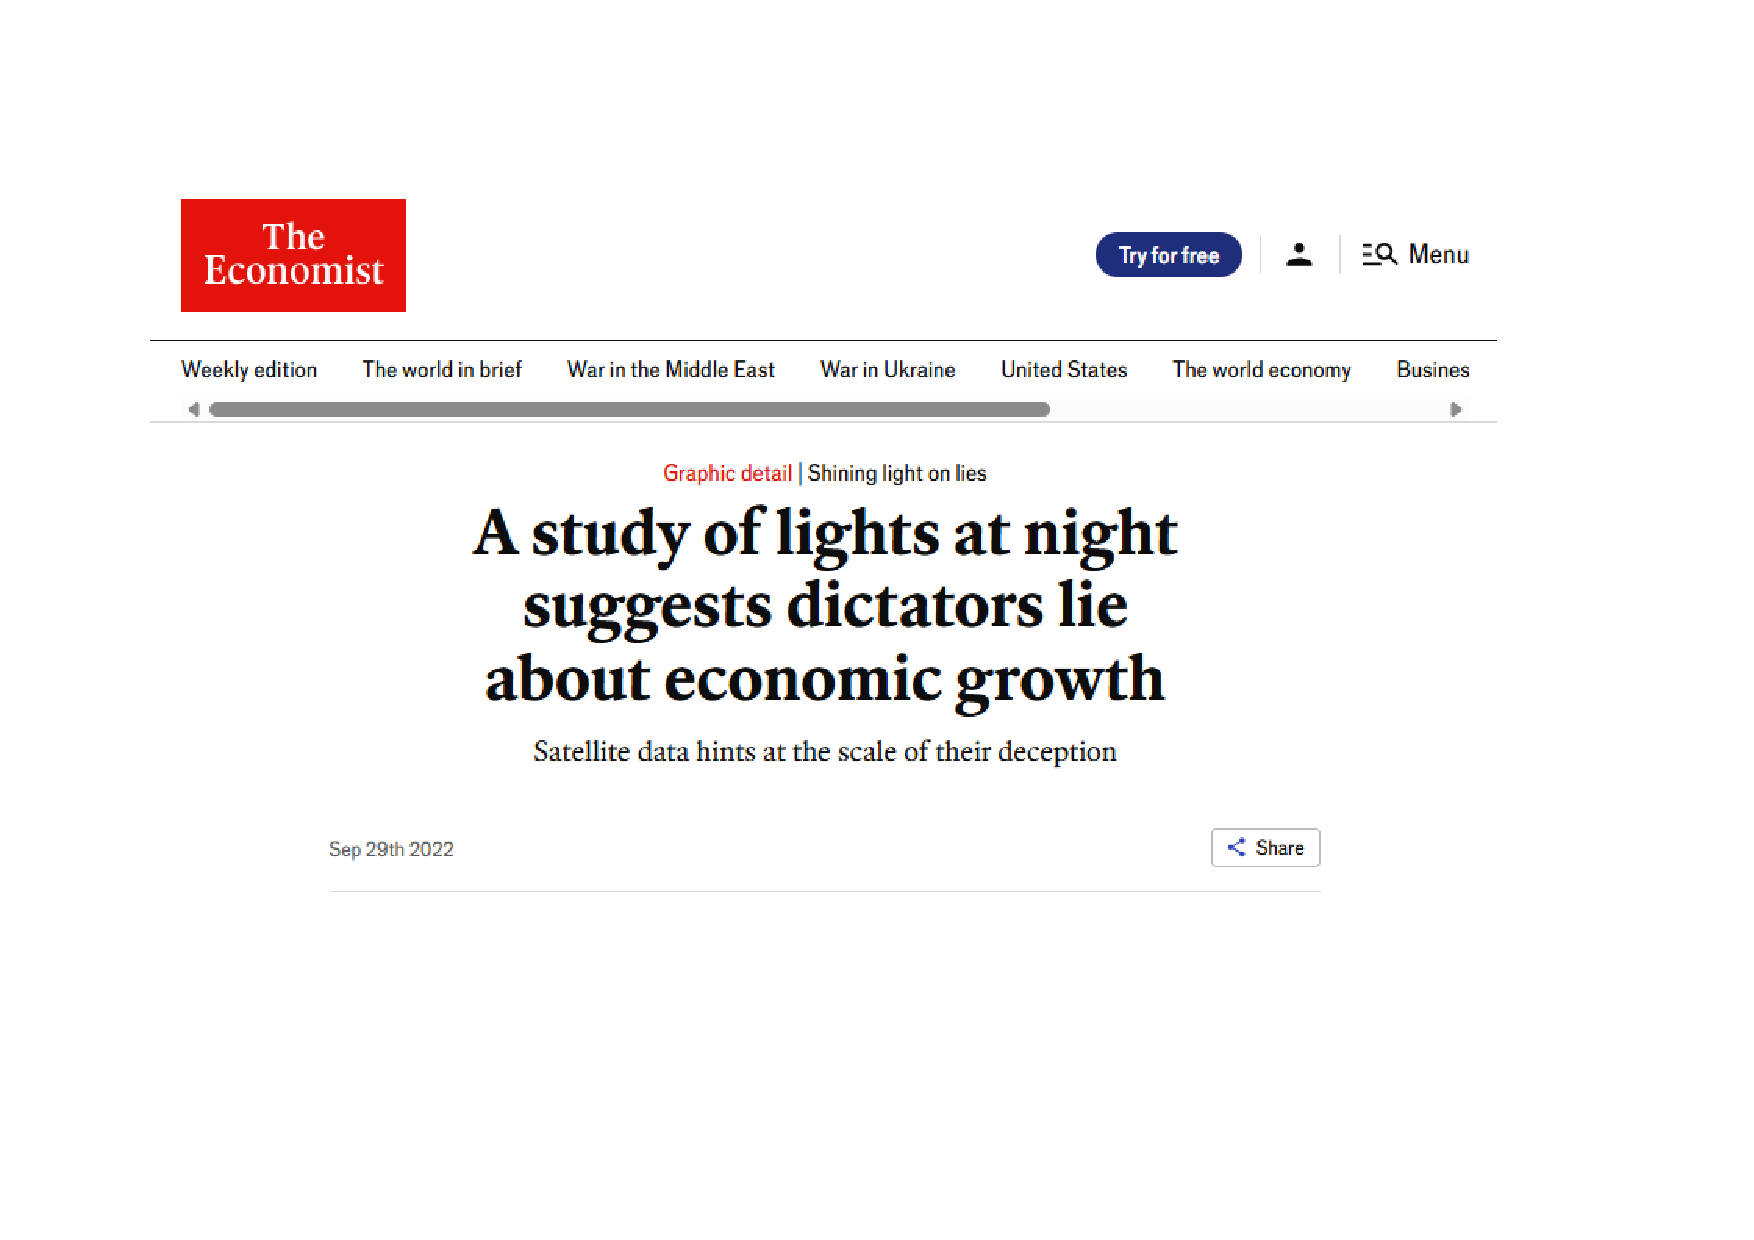
\includegraphics[width=0.7\linewidth]{Figs/economist} \end{center}
\vspace{0.2cm}
\begin{center}
\tiny
\url{https://www.economist.com/graphic-detail/2022/09/29/a-study-of-lights-at-night-suggests-dictators-lie-about-economic-growth}
\end{center}
\end{frame}

\begin{frame}
\begin{center}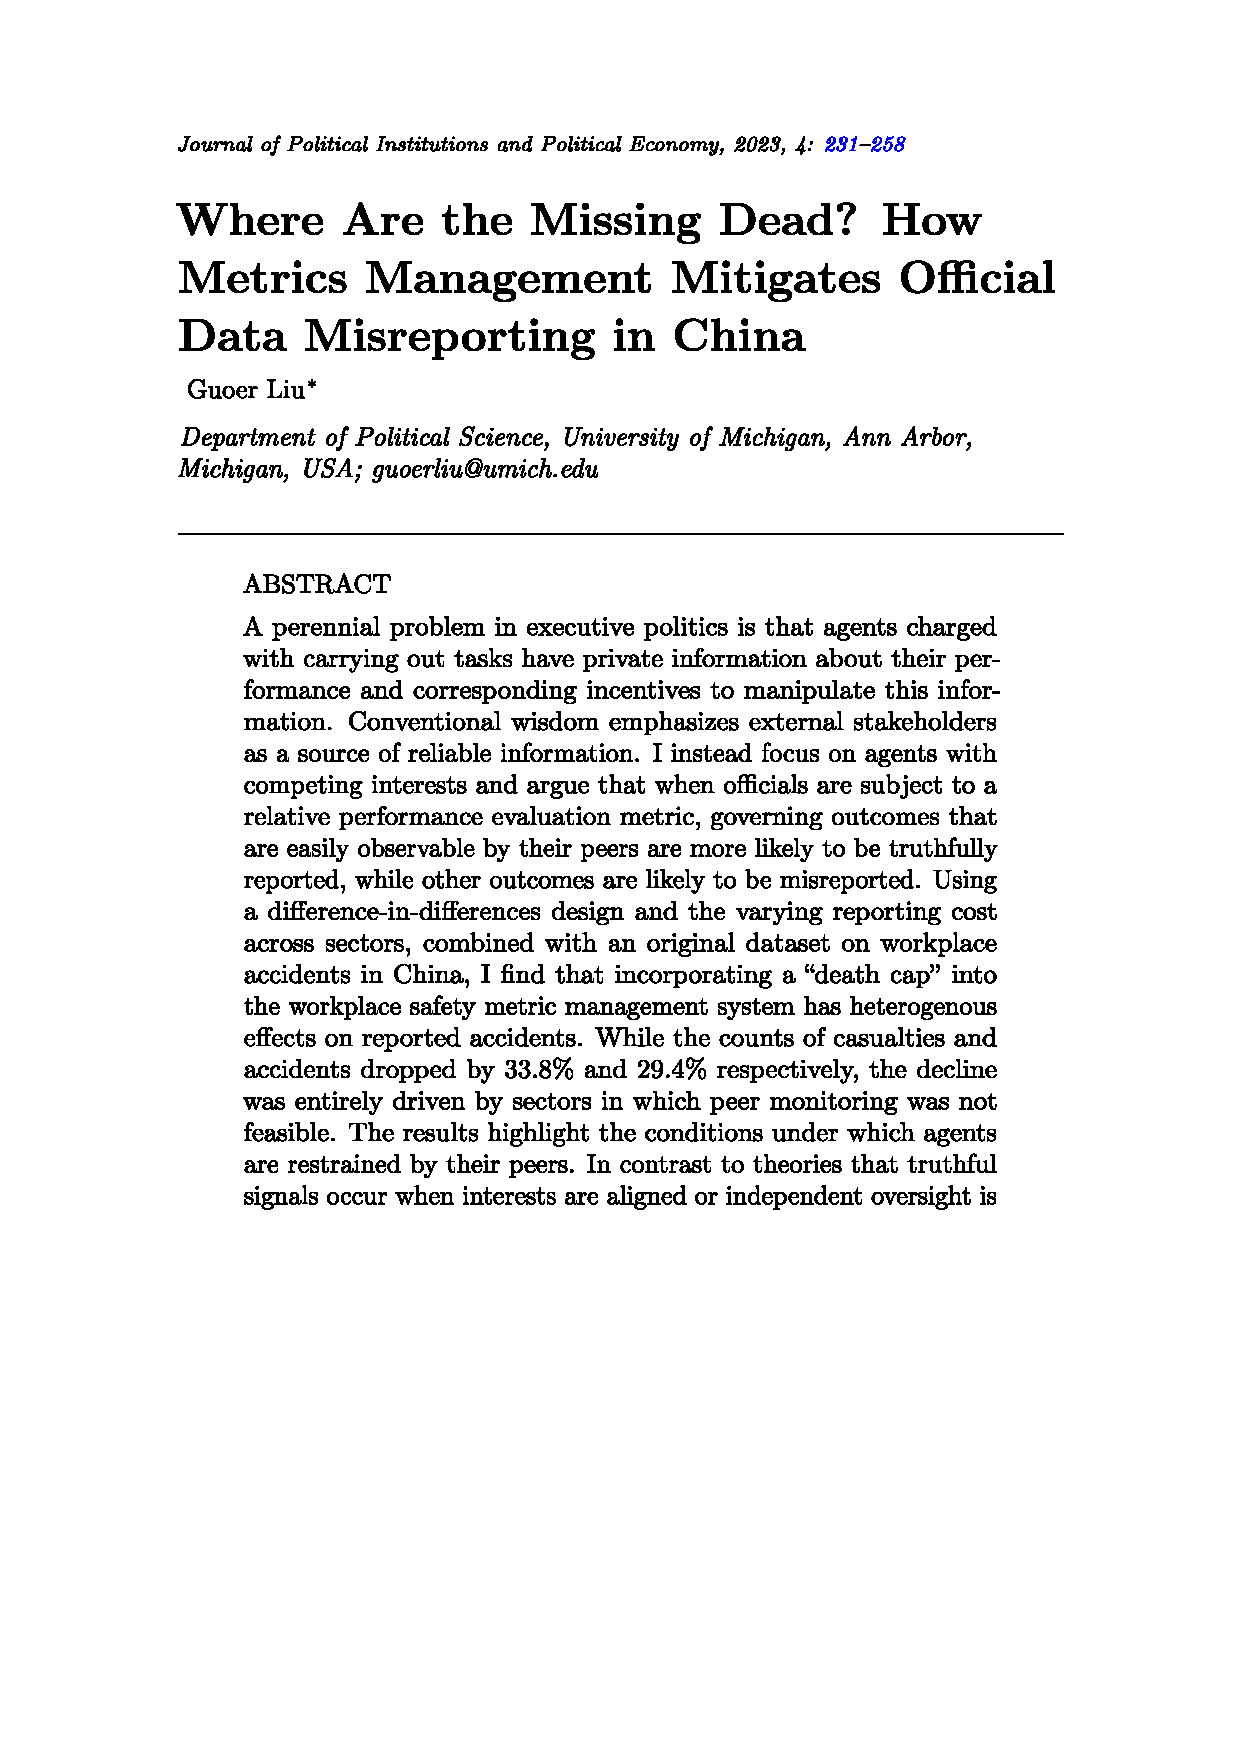
\includegraphics[width=0.6\linewidth]{Figs/liu_cover} \end{center}
\end{frame}

\begin{frame}
\begin{center}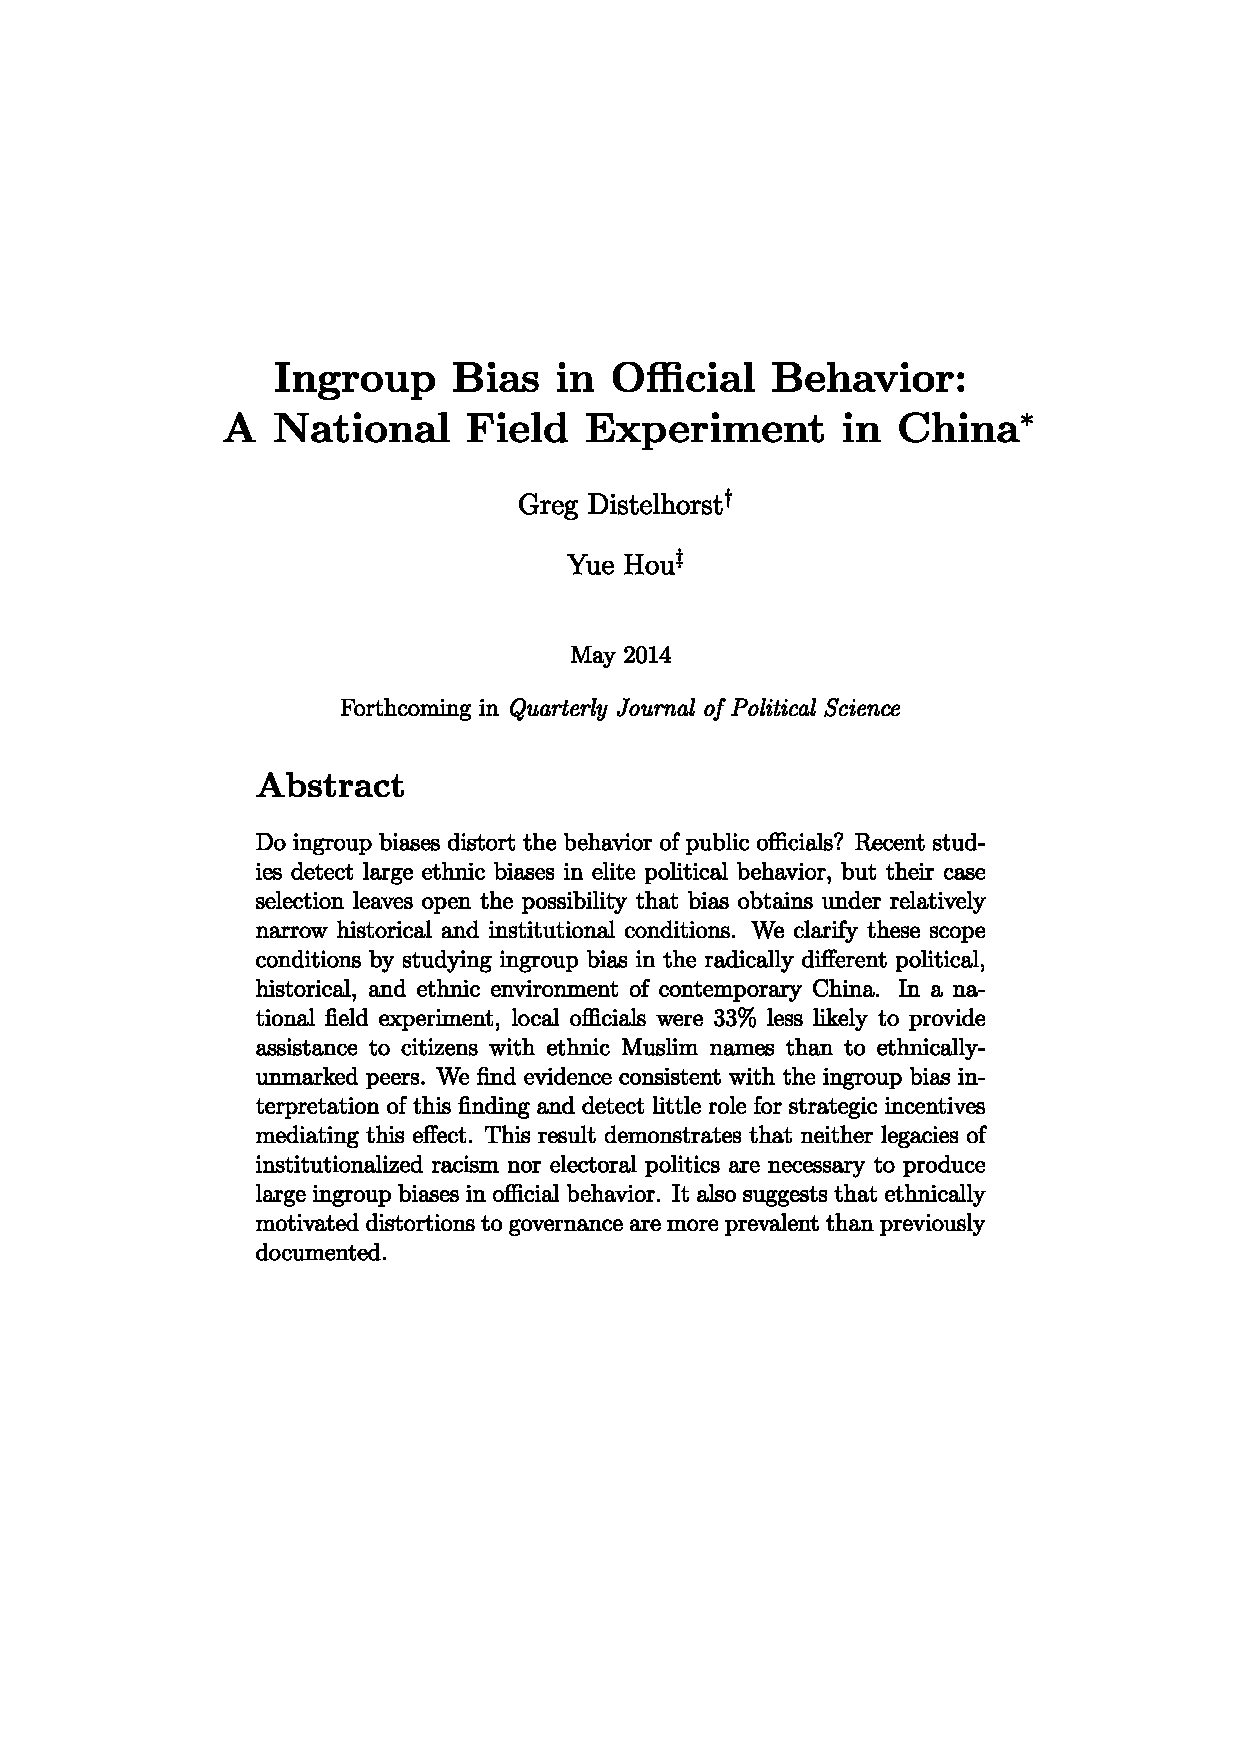
\includegraphics[width=0.7\linewidth]{Figs/Examples/hou_cover} \end{center}
\end{frame}

\begin{frame}{Past and current research}
\phantomsection\label{past-and-current-research}
\begin{itemize}
  \item Governance and development in multiethnic China
  \vspace{0.1cm}
  \begin{itemize}
    \item Rethinking the politics of ethnic local autonomy (book project)
    \item Poverty alleviation and local state-building in peripheral provinces (\textit{JJPS} 2021)
    \item Ethnic empowerment and environmental governance
    \item Dualilty of ethnic descriptive representation
  \end{itemize}
  \vspace{0.2cm}
  \item Using AI tools to (re)mapping the information network of political elites
  \vspace{0.2cm}
  \item Using court records to study administrative litigation, with \textbf{Haibo He} (Tsinghua) and \textbf{Chao Ma} (UIBE)
  \vspace{0.2cm}
  \item Multilevel agenda setting in times of crisis: A text-as-data approach, with \textbf{Tao Lin} (University of Washington)
\end{itemize}
\end{frame}

\begin{frame}{Concluding remarks}
\phantomsection\label{concluding-remarks}
\begin{itemize}
  \item Find out \textbf{who you are} and \textbf{what you want to be and do} -- your decision may depend on where you are (or going back to history)
  \vspace{0.6cm}
  \item Curate the skills you need -- be \textbf{selectively thorough}
  \vspace{0.6cm}
  \item Find those who can support and collaborate with you -- engage in \textbf{interdisciplinary knowledge co-production}
  \vspace{0.6cm}
  \item Read broadly -- \textbf{go beyond political science and (mainland) China} to gain inspiration and a broader comparative perspective
\end{itemize}
\end{frame}

\begin{frame}
\vspace{0.7cm}

Thank you!\\
\vspace{0.7cm} \texttt{c.cheng@bbk.ac.uk}
\end{frame}

\begin{frame}{Rethinking the politics of ethnic local autonomy}
\phantomsection\label{rethinking-the-politics-of-ethnic-local-autonomy}
\begin{itemize}
  \item Why do the Communist Party of China grant \textbf{ethnic local autonomy}?
  \vspace{0.5cm}
  \item When and where will the Center designate \textbf{ethnic autonomous territories} (EATs)?
  \vspace{0.5cm}
  \item How can local (policy/administrative) decentralization contribute to nation-state building?
\end{itemize}
\end{frame}

\begin{frame}{Rethinking the politics of ethnic local autonomy}
\phantomsection\label{rethinking-the-politics-of-ethnic-local-autonomy-1}
\begincols
\begincol{.43\textwidth}
  \begin{small}
  \begin{itemize}
  \item \textbf{Archival research} in the US, Hong Kong and China
  \vspace{0.35cm}
  \item \textbf{Elite interviews}: Conversations with Han and non-Han cadres at the central and local levels across different provinces
  \vspace{0.35cm}
  \item \textbf{Process-tracing and QCA}: Structured process tracing the designation of ethnic autonomous prefectures
  \end{itemize}
  \end{small}
  \endcol
  \begincol{.5\textwidth}
  \vspace{0.5cm}
  \begin{figure}
  \centering
  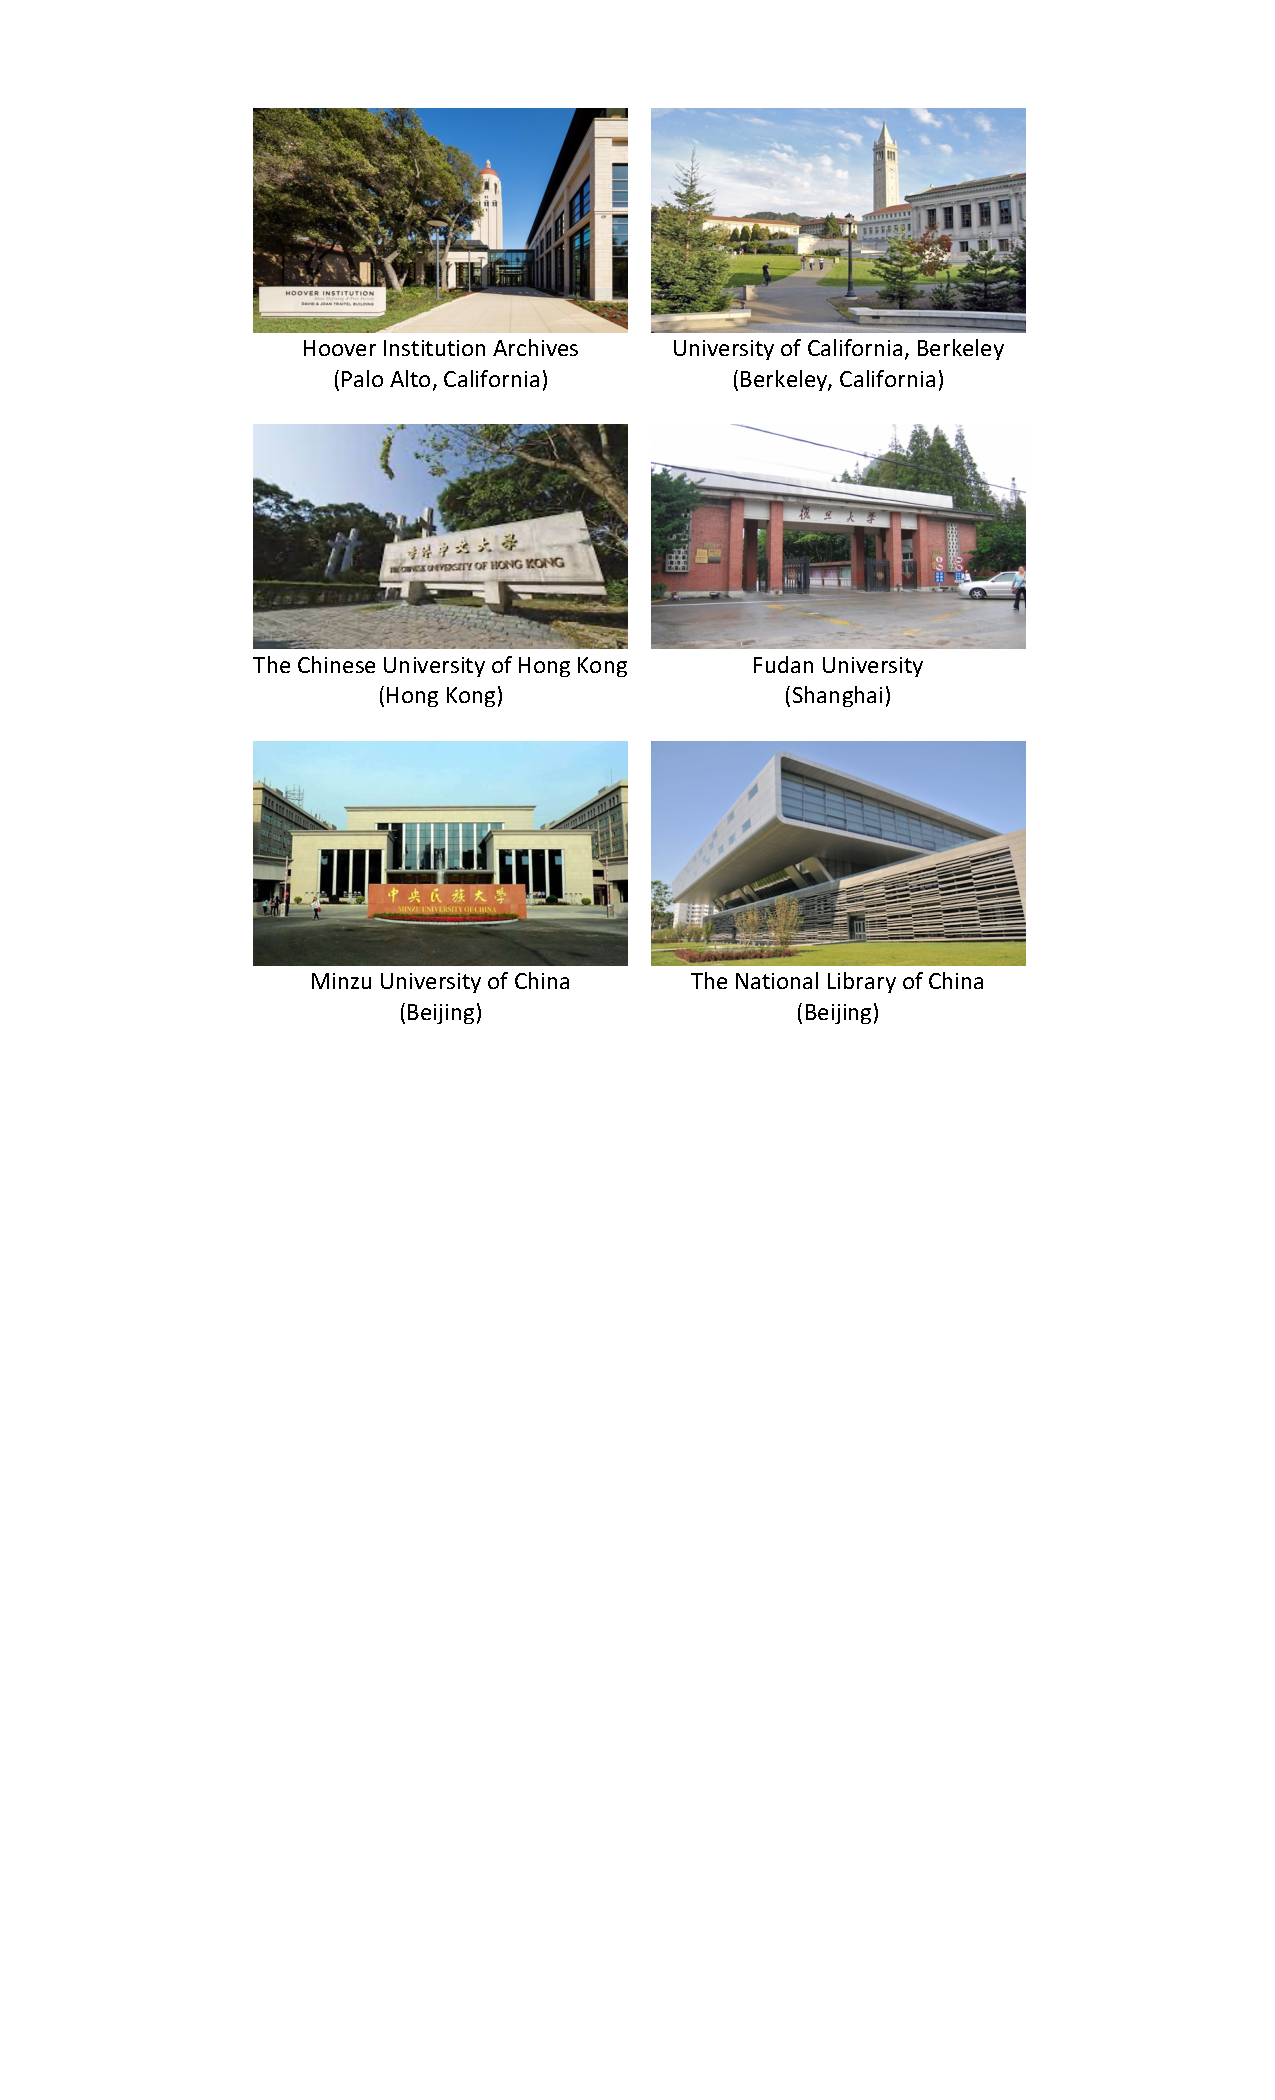
\includegraphics[scale=0.43]{Figs/sites_6}
  \end{figure}
  \endcol
\endcols
\end{frame}

\begin{frame}{Rethinking the politics of ethnic local autonomy}
\phantomsection\label{rethinking-the-politics-of-ethnic-local-autonomy-2}
\begin{itemize}
  \item \textbf{Supervised machine learning} and \textbf{social network analysis}: Capturing the \textit{connectedness} and \textit{network structure} among/between central and local cadres based on an original biographical dataset of Chinese political elites (1949-2003)
  \begin{itemize}
    \item Between the pair of cadres, I create the indices of \textbf{connectedness} based on their \textbf{biographical similarity}
    \begin{figure}
    \centering
    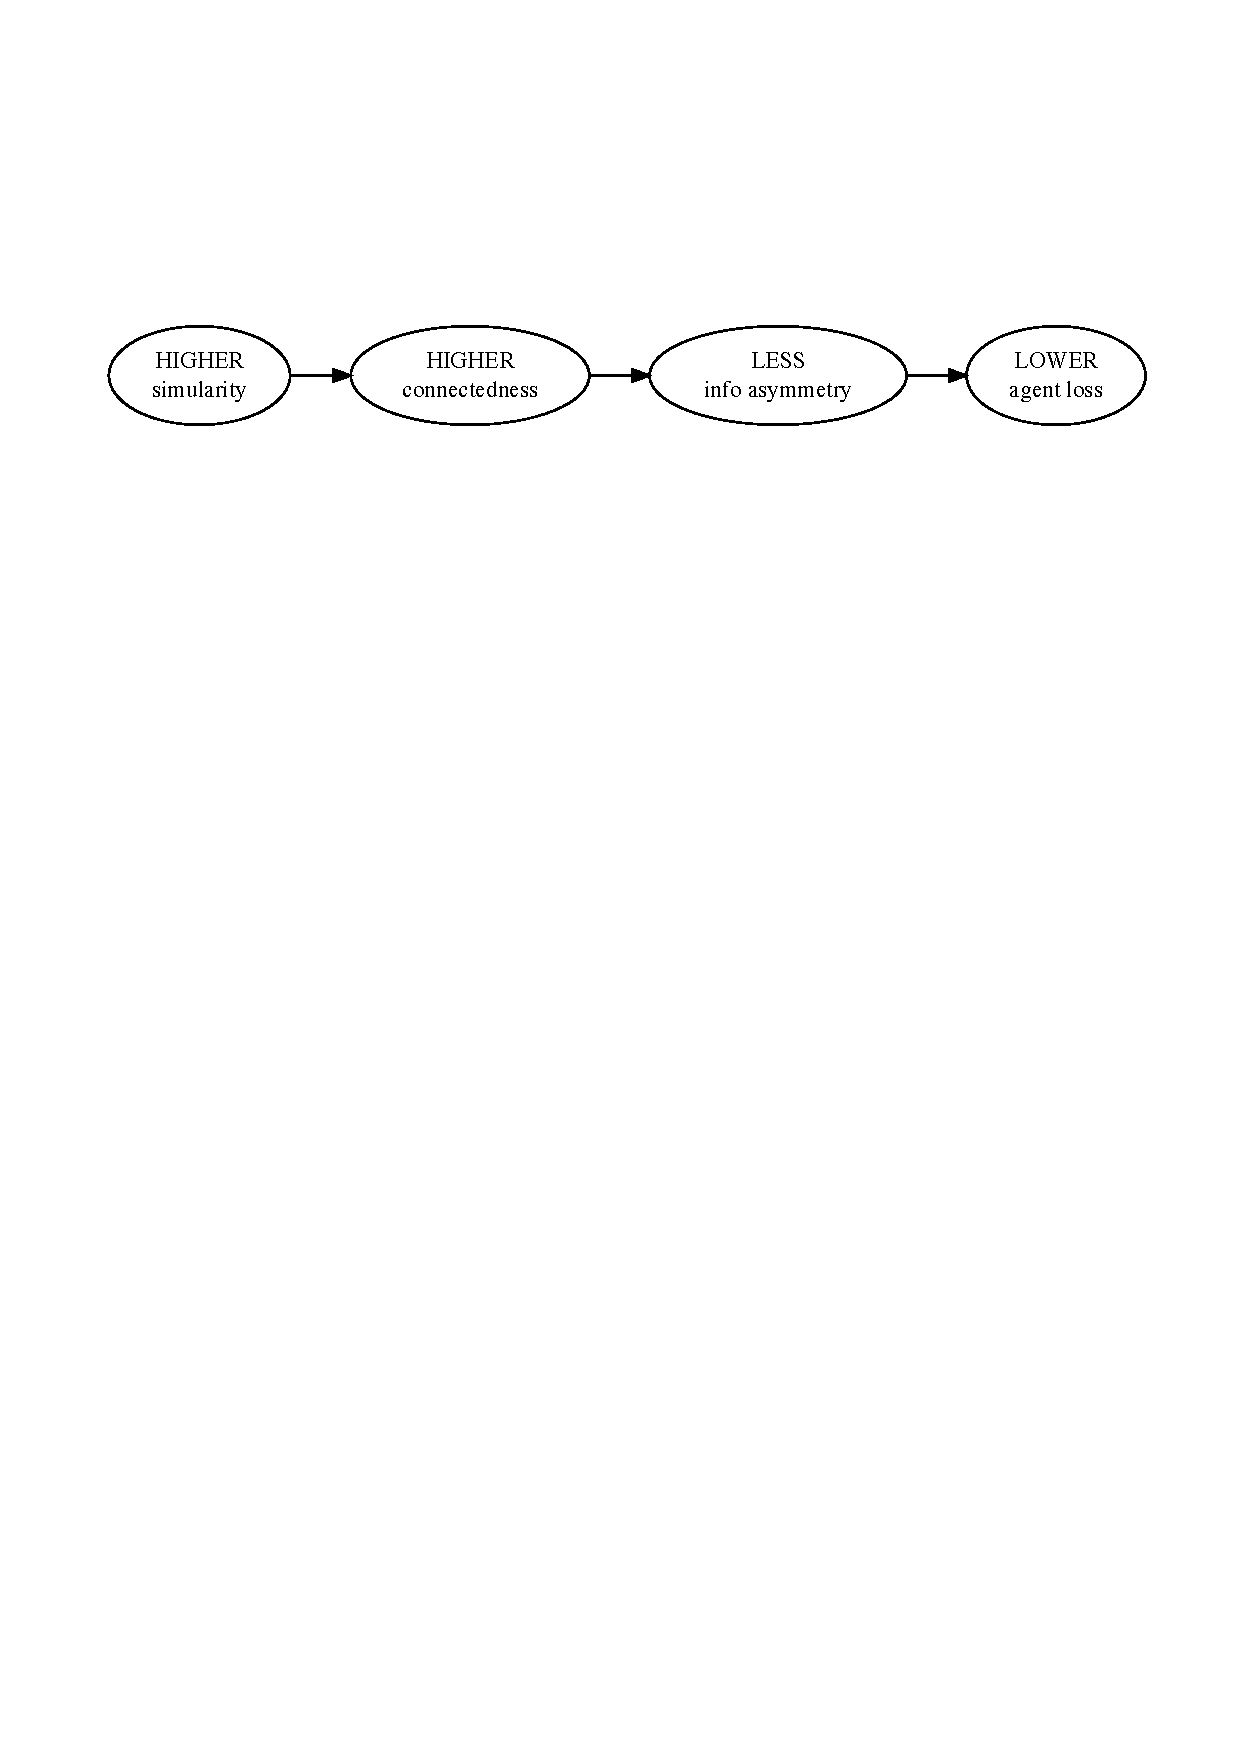
\includegraphics[scale=0.52]{Figs/cpen}
    \end{figure}
    \item The same connectedness measure can be used to construct the information network of Politburo members and measure the degree of \textbf{central leadership fragmentation} by \textbf{community detection}
  \end{itemize}
  \vspace{0.3cm}
  \item \textbf{Multivariate regression}: Modeling the number of active EATs as a function of different network structural indicators
\end{itemize}
\end{frame}

\begin{frame}{Rethinking the politics of ethnic local autonomy}
\phantomsection\label{rethinking-the-politics-of-ethnic-local-autonomy-3}
\begin{itemize}
  \item Ethnic local autonomy acts as an \textbf{institution of agent control}
\end{itemize}
\vspace{0.2cm}
\begin{figure}
  \center
  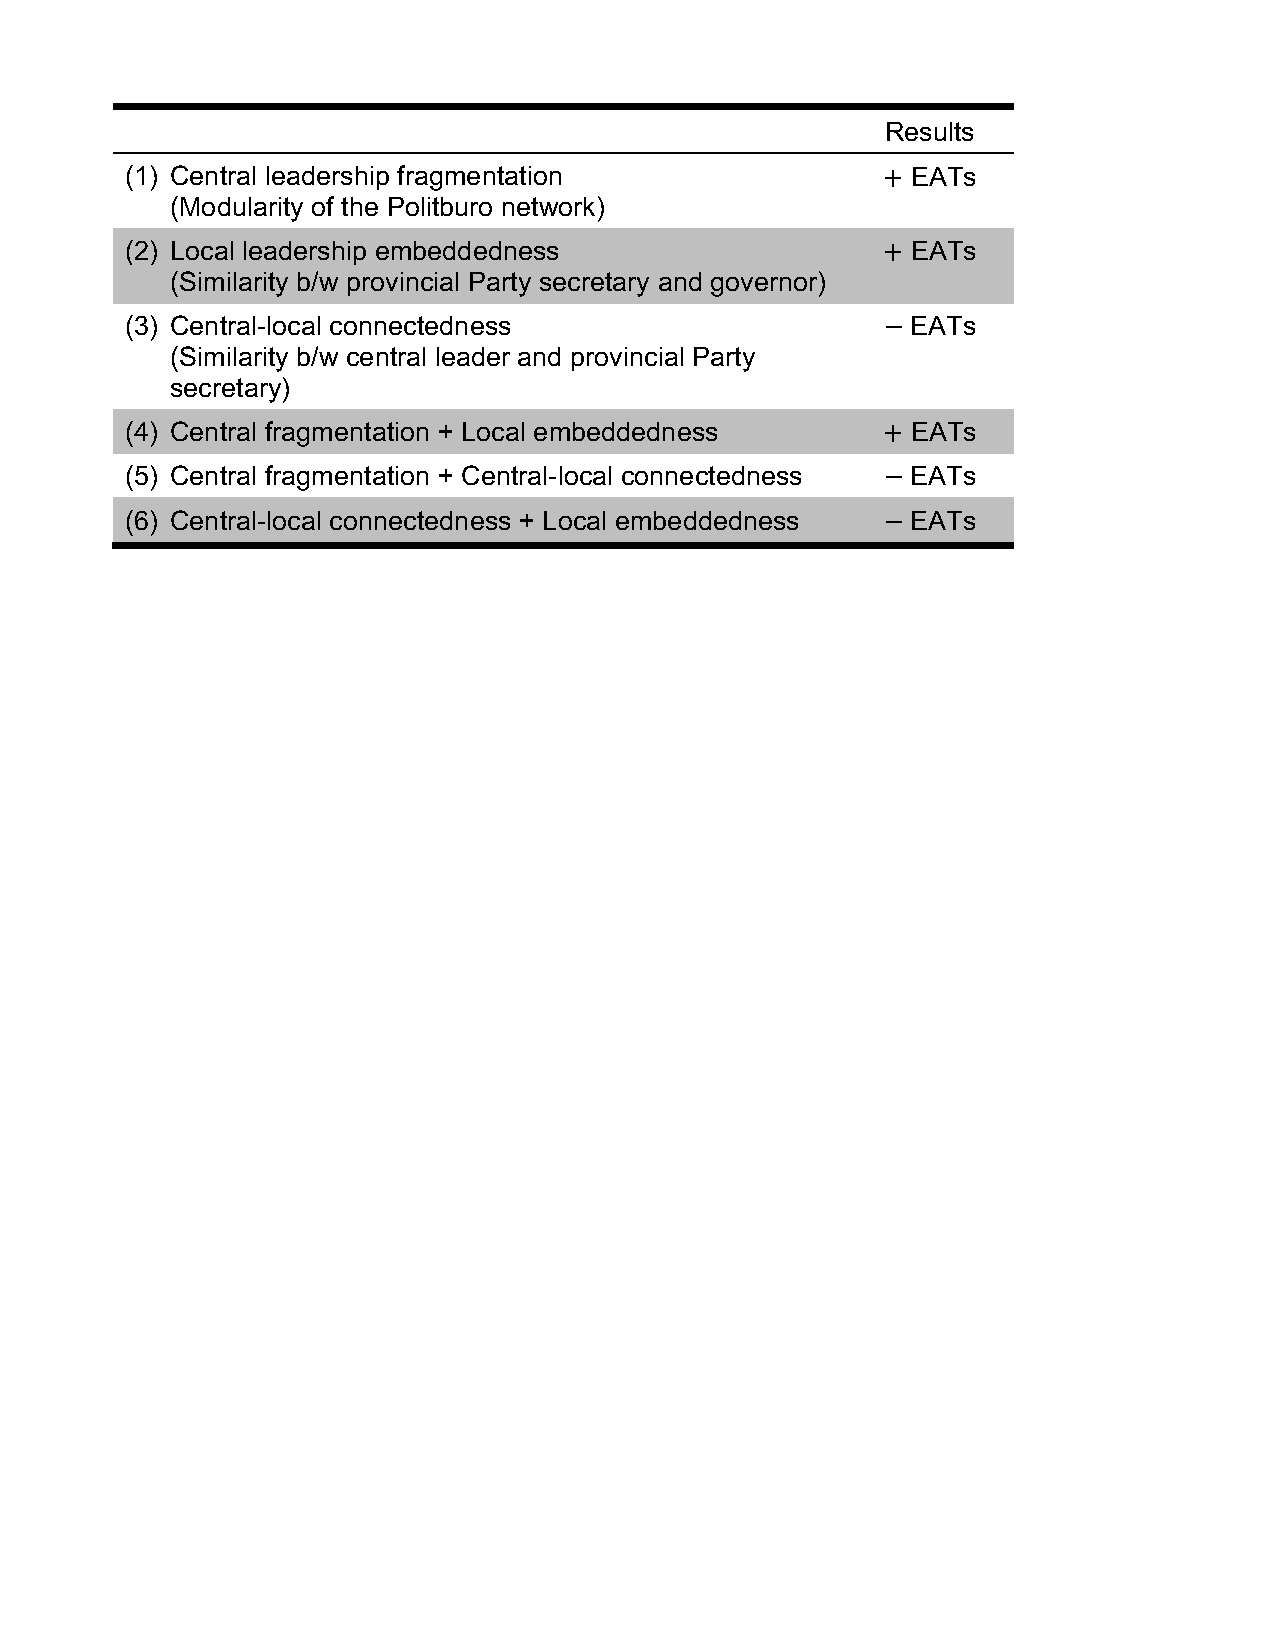
\includegraphics[scale=0.5]{Figs/findings}
\end{figure}
\end{frame}

\begin{frame}{Rethinking the politics of ethnic local autonomy}
\phantomsection\label{rethinking-the-politics-of-ethnic-local-autonomy-4}
\begin{itemize}
  \item EATs act as \textbf{enclaves} that constrain the power of provincial elites
  \vspace{0.3cm}
  \begin{itemize}
    \item Sub-provincial EATs are \textbf{more} likely to pass and revise autonomous regulations when the provincial elites are potentially defiant
    \vspace{0.2cm}
    \item Ruling non-Han cadres in sub-provincial EATs are \textbf{less} likely to have worked at the provincial level prior to their appointments
  \end{itemize}
\end{itemize}
\end{frame}

\begin{frame}{Rethinking the politics of ethnic local autonomy}
\phantomsection\label{rethinking-the-politics-of-ethnic-local-autonomy-5}
\begin{itemize}
  \item Going \textbf{cross-national}: Post-WWII authoritarian regimes are more likely to introduce regional autonomy to ethnic minorities when their ruling power is contested within the inner circle
  \vspace{0.6cm}
  \item Going back to \textbf{history}: Post-civil war \textit{decentralization} and \textit{state power consolidation} in imperial and Republican China
  \vspace{0.2cm}
  \begin{itemize}
    \item Western Han dynasty (202 BC–220 AD): Kingdoms and marquis states
    \item The Kuomintang (KMT) regime (1928-1949 AD): Countering recalcitrant provincial warlords through the county-level self-government movement
  \end{itemize}
\end{itemize}
\end{frame}

\begin{frame}{(Re)mapping the information network of political elites}
\phantomsection\label{remapping-the-information-network-of-political-elites}
\begin{itemize}
  \item The focus on "high-politics" in the literature on Communist regimes: The absence of independent, strong formal institutions has pushed researchers have to focus on prominent political elites in authoritarian regimes
  \vspace{0.3cm}
  \item \textbf{Factionalism} is one of the most researched topics in the Chinese politics literature (e.g., Nathan 1973; Tsou 1976; Pye 1981; Dittmer 2002; Huang 2006; Bo 2007; Shih et al 2012)
  \vspace{0.3cm}
  \item The power struggles and cooperation between different factions or "informal" groups have been considered as the main driving forces for policy and political changes in the country
\end{itemize}
\end{frame}

\begin{frame}{(Re)mapping the information network of political elites}
\phantomsection\label{remapping-the-information-network-of-political-elites-1}
\begin{itemize}
  \item Create the timeline of key life events of each cadre using public biographic information
  \vspace{0.1cm}
  \begin{itemize}
    \item Demographic characteristics (e.g., birth year and provincial origin)
    \item Educational background (e.g., colleges and universities)
    \item Political career (e.g., involvement in key events between 1921 and 1949; Party and government posts after 1949)
  \end{itemize}
  \vspace{0.2cm}
  \item Create the (decomposed) \textbf{\textit{attribute vector}} of a cadre based on her/her timeline and measure the distance/similarity between a pair of attribute vectors in the multidimensional space
  \vspace{0.1cm}
  \begin{itemize}
    \item Time: Are the cadres of interest both alive in a given year?
    \item Location: Are they both at the same location in a given year?
    \item Activity: Are they working in the same department/unit in a given year?
  \end{itemize}
\end{itemize}
\end{frame}

\begin{frame}{(Re)mapping the information network of political elites}
\phantomsection\label{remapping-the-information-network-of-political-elites-2}
\begin{figure}
\centering
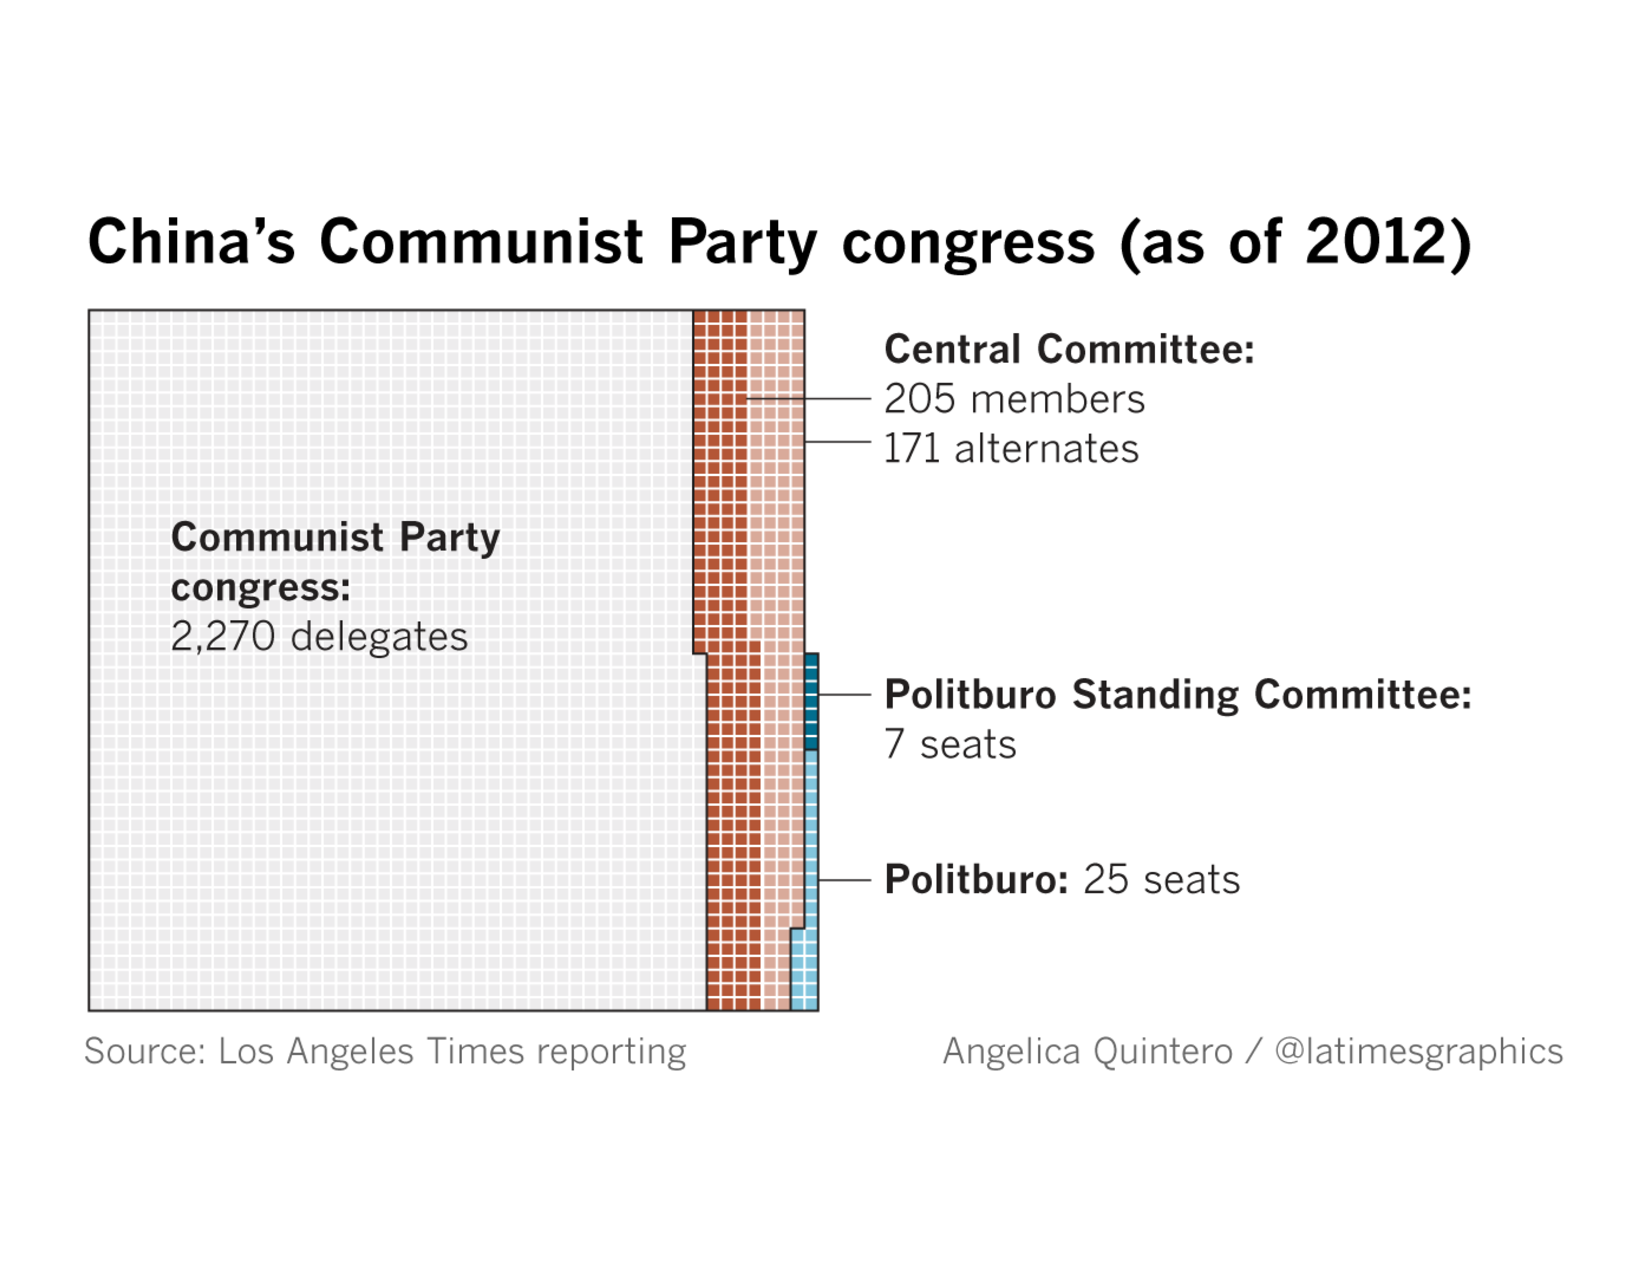
\includegraphics[scale=0.26]{Figs/selection}
\end{figure}
\vspace{0.3cm}
\begin{itemize}
  \item Use \textbf{variable selection} (elastic net regularization and other methods) to identify the key biographical variables in CC of each year when measuring biographical similarity
  \vspace{0.1cm}
  \item Use \textbf{community detection} to assess the degree to which a Politburo network can be divided
\end{itemize}
\end{frame}

\begin{frame}{Using court records to study admin litigation}
\phantomsection\label{using-court-records-to-study-admin-litigation}
The release of \textbf{China Judgements Online}
(\url{https://wenshu.court.gov.cn/}) made a crucial breakthrough in the
empirical legal studies in China (Ma, Yu and He 2016; Liebman et al
2020). \vspace{0.2cm}

\begin{center}
\includegraphics[width=0.65\linewidth]{Figs/wenshu_crop} \end{center}
\end{frame}

\begin{frame}{Using court records to study admin litigation}
\phantomsection\label{using-court-records-to-study-admin-litigation-1}
\begin{itemize}
  \item \textbf{Question}: Are the local courts more likely stand with the citizens following the reforms?
  \vspace{0.2cm}
  \begin{itemize}
    \item Railway transport courts (\textit{China Review} 2022)
    \item Case registration system
    \item Elevated and off-site trials
  \end{itemize}
  \vspace{0.6cm}
  \item \textbf{Extensions}
  \vspace{0.2cm}
  \begin{itemize}
    \item Who do the citizens go to the courts? A national \textbf{conjoint} experiment
    \item Local dynamics of judicial decision-making: A \textbf{text-as-data} approach
  \end{itemize}
\end{itemize}
\end{frame}

\end{document}
